% -*- Mode:TeX -*-

%% IMPORTANT: The official thesis specifications are available at:
%%            http://libraries.mit.edu/archives/thesis-specs/
%%
%%            Please verify your thesis' formatting and copyright
%%            assignment before submission.  If you notice any
%%            discrepancies between these templates and the 
%%            MIT Libraries' specs, please let us know
%%            by e-mailing thesis@mit.edu

%% The documentclass options along with the pagestyle can be used to generate
%% a technical report, a draft copy, or a regular thesis.  You may need to
%% re-specify the pagestyle after you \include  cover.tex.  For more
%% information, see the first few lines of mitthesis.cls. 

%\documentclass[12pt,vi,twoside]{mitthesis}
%%
%%  If you want your thesis copyright to you instead of MIT, use the
%%  ``vi'' option, as above.
%%
%\documentclass[12pt,twoside,leftblank]{mitthesis}
%%
%% If you want blank pages before new chapters to be labelled ``This
%% Page Intentionally Left Blank'', use the ``leftblank'' option, as
%% above. 

\documentclass[12pt,twoside,leftblank]{mitthesis}
\usepackage{lgrind}
%% These have been added at the request of the MIT Libraries, because
%% some PDF conversions mess up the ligatures.  -LB, 1/22/2014
\usepackage{cmap}
\usepackage[T1]{fontenc}
%% Package "lmodern" added by user request see ServiceNow INC0396734 -OT, 4/29/2020
\usepackage{lmodern}

%% For code snippets
\usepackage{listings}
\usepackage{listings-golang} % Installed locally
\usepackage{color}

\lstset{ % add your own preferences
    frame=single,
    basicstyle=\footnotesize\ttfamily,
    keywordstyle=\color{red},
    numbers=left,
    numbersep=5pt,
    showstringspaces=false, 
    stringstyle=\color{blue},
    tabsize=4,
    language=Golang, % this is it !
    captionpos=b, % sets the caption-position to bottom
}

\renewcommand\lstlistingname{Code Snippet}
\renewcommand{\lstlistlistingname}{Code Snippets}

\usepackage{graphicx}
\graphicspath{ {./images/} }

\usepackage{enumitem}

\usepackage{array}

\usepackage{url}

\pagestyle{plain}

\renewcommand{\arraystretch}{1.7}

\newcommand{\sys}{{Felix}} 

%% This bit allows you to either specify only the files which you wish to
%% process, or `all' to process all files which you \include.
%% Krishna Sethuraman (1990).

%% \typein [\files]{Enter file names to process, (chap1,chap2 ...), or `all' to
%% process all files:}
%% \def\all{all}
%% \ifx\files\all \typeout{Including all files.} \else \typeout{Including only \files.} \includeonly{\files} \fi

\begin{document}

% -*-latex-*-
% 
% For questions, comments, concerns or complaints:
% thesis@mit.edu
% 
%
% $Log: cover.tex,v $
% Revision 1.8  2008/05/13 15:02:15  jdreed
% Degree month is June, not May.  Added note about prevdegrees.
% Arthur Smith's title updated
%
% Revision 1.7  2001/02/08 18:53:16  boojum
% changed some \newpages to \cleardoublepages
%
% Revision 1.6  1999/10/21 14:49:31  boojum
% changed comment referring to documentstyle
%
% Revision 1.5  1999/10/21 14:39:04  boojum
% *** empty log message ***
%
% Revision 1.4  1997/04/18  17:54:10  othomas
% added page numbers on abstract and cover, and made 1 abstract
% page the default rather than 2.  (anne hunter tells me this
% is the new institute standard.)
%
% Revision 1.4  1997/04/18  17:54:10  othomas
% added page numbers on abstract and cover, and made 1 abstract
% page the default rather than 2.  (anne hunter tells me this
% is the new institute standard.)
%
% Revision 1.3  93/05/17  17:06:29  starflt
% Added acknowledgements section (suggested by tompalka)
% 
% Revision 1.2  92/04/22  13:13:13  epeisach
% Fixes for 1991 course 6 requirements
% Phrase "and to grant others the right to do so" has been added to 
% permission clause
% Second copy of abstract is not counted as separate pages so numbering works
% out
% 
% Revision 1.1  92/04/22  13:08:20  epeisach

% NOTE:
% These templates make an effort to conform to the MIT Thesis specifications,
% however the specifications can change.  We recommend that you verify the
% layout of your title page with your thesis advisor and/or the MIT 
% Libraries before printing your final copy.
\title{Titles Goes Here}

\author{Damian Barabonkov}
\prevdegrees{B.S., Massachusetts Institute of Technology (2020)}
% If you wish to list your previous degrees on the cover page, use the 
% previous degrees command:
%       \prevdegrees{A.A., Harvard University (1985)}
% You can use the \\ command to list multiple previous degrees
%       \prevdegrees{B.S., University of California (1978) \\
%                    S.M., Massachusetts Institute of Technology (1981)}
\department{Department of Electrical Engineering and Computer Science}

% If the thesis is for two degrees simultaneously, list them both
% separated by \and like this:
% \degree{Doctor of Philosophy \and Master of Science}
\degree{Master of Engineering in Computer Science and Engineering}

% As of the 2007-08 academic year, valid degree months are September, 
% February, or June.  The default is June.
\degreemonth{May}
\degreeyear{2021}
\thesisdate{May 14, 2021}

%% By default, the thesis will be copyrighted to MIT.  If you need to copyright
%% the thesis to yourself, just specify the `vi' documentclass option.  If for
%% some reason you want to exactly specify the copyright notice text, you can
%% use the \copyrightnoticetext command.  
%\copyrightnoticetext{\copyright IBM, 1990.  Do not open till Xmas.}

% If there is more than one supervisor, use the \supervisor command
% once for each.
\supervisor{Anish Athalye}{Doctoral Candidate}
\supervisor{M. Frans Kaashoek}{Charles Piper Professor}

% This is the department committee chairman, not the thesis committee
% chairman.  You should replace this with your Department's Committee
% Chairman.
\chairman{Katrina LaCurts}{Chair, Master of Engineering Thesis Committee}

% Make the titlepage based on the above information.  If you need
% something special and can't use the standard form, you can specify
% the exact text of the titlepage yourself.  Put it in a titlepage
% environment and leave blank lines where you want vertical space.
% The spaces will be adjusted to fill the entire page.  The dotted
% lines for the signatures are made with the \signature command.
\maketitle

% The abstractpage environment sets up everything on the page except
% the text itself.  The title and other header material are put at the
% top of the page, and the supervisors are listed at the bottom.  A
% new page is begun both before and after.  Of course, an abstract may
% be more than one page itself.  If you need more control over the
% format of the page, you can use the abstract environment, which puts
% the word "Abstract" at the beginning and single spaces its text.

%% You can either \input (*not* \include) your abstract file, or you can put
%% the text of the abstract directly between the \begin{abstractpage} and
%% \end{abstractpage} commands.

% First copy: start a new page, and save the page number.
\cleardoublepage
% Uncomment the next line if you do NOT want a page number on your
% abstract and acknowledgments pages.
% \pagestyle{empty}
\setcounter{savepage}{\thepage}
\begin{abstractpage}
% $Log: abstract.tex,v $
% Revision 1.1  93/05/14  14:56:25  starflt
% Initial revision
% 
% Revision 1.1  90/05/04  10:41:01  lwvanels
% Initial revision
% 
%
%% The text of your abstract and nothing else (other than comments) goes here.
%% It will be single-spaced and the rest of the text that is supposed to go on
%% the abstract page will be generated by the abstractpage environment.  This
%% file should be \input (not \include 'd) from cover.tex.
Transaction authentication is an attractive extension to typical two-factor authentication. It is proposed by the World-Wide-Web Consortium (W3C) as a mechanism to secure individual ``high-risk'' operations of a website by requiring attestation from a hardware authenticator device. It defends against a strict threat model where an adversary may have complete control of all infrastructure components: the host computer, operating system, web-browser, network, etc. 

Unfortunately, transaction authentication as defined by the W3C is not widely adopted. Typical means for supporting transaction authentication in a web service involve significant modifications to its codebase. This approach comes with a degree of complexity which is error-prone and difficult to develop and maintain.

%% 
%% \iffalse
%% is difficult to develop, maintain and is error-prone due to the entailed complexity.
%% \fi
%% 

This thesis presents a firewall system for integrating transaction authentication into a new or existing web service. The aim is to lower the barriers preventing its adoption. An engineer would need to populate a configuration file for the firewall and make relatively few code changes to the web service to integrate transaction authentication. The firewall intercepts all HTTP traffic sent to the web service. Based on the configuration, any requests deemed innocuous are proxied directly to the web service. All other requests are considered high-risk and are held back and validated using transaction authentication. Only if the validation passes are they also permitted to pass through to the web service.

This thesis evaluates the footprint and complexity of the firewall approach. It is close to 8 times more concise than the typical means for integrating transaction authentication in a web service. This entails easier development and fewer opportunities for accidental bugs or errors in the code. However, there is an associated latency of at worst 1.5x slower when using the firewall under heavy concurrent load.

\end{abstractpage}

% Additional copy: start a new page, and reset the page number.  This way,
% the second copy of the abstract is not counted as separate pages.
% Uncomment the next 6 lines if you need two copies of the abstract
% page.
% \setcounter{page}{\thesavepage}
% \begin{abstractpage}
% % $Log: abstract.tex,v $
% Revision 1.1  93/05/14  14:56:25  starflt
% Initial revision
% 
% Revision 1.1  90/05/04  10:41:01  lwvanels
% Initial revision
% 
%
%% The text of your abstract and nothing else (other than comments) goes here.
%% It will be single-spaced and the rest of the text that is supposed to go on
%% the abstract page will be generated by the abstractpage environment.  This
%% file should be \input (not \include 'd) from cover.tex.
Transaction authentication is an attractive extension to typical two-factor authentication. It is proposed by the World-Wide-Web Consortium (W3C) as a mechanism to secure individual ``high-risk'' operations of a website by requiring attestation from a hardware authenticator device. It defends against a strict threat model where an adversary may have complete control of all infrastructure components: the host computer, operating system, web-browser, network, etc. 

Unfortunately, transaction authentication as defined by the W3C is not widely adopted. Typical means for supporting transaction authentication in a web service involve significant modifications to its codebase. This approach comes with a degree of complexity which is error-prone and difficult to develop and maintain.

%% 
%% \iffalse
%% is difficult to develop, maintain and is error-prone due to the entailed complexity.
%% \fi
%% 

This thesis presents a firewall system for integrating transaction authentication into a new or existing web service. The aim is to lower the barriers preventing its adoption. An engineer would need to populate a configuration file for the firewall and make relatively few code changes to the web service to integrate transaction authentication. The firewall intercepts all HTTP traffic sent to the web service. Based on the configuration, any requests deemed innocuous are proxied directly to the web service. All other requests are considered high-risk and are held back and validated using transaction authentication. Only if the validation passes are they also permitted to pass through to the web service.

This thesis evaluates the footprint and complexity of the firewall approach. It is close to 8 times more concise than the typical means for integrating transaction authentication in a web service. This entails easier development and fewer opportunities for accidental bugs or errors in the code. However, there is an associated latency of at worst 1.5x slower when using the firewall under heavy concurrent load.

% \end{abstractpage}

\cleardoublepage

\section*{Acknowledgments}

TODO: Acknowledgments go here!

parents, unrelenting support.

%%%%%%%%%%%%%%%%%%%%%%%%%%%%%%%%%%%%%%%%%%%%%%%%%%%%%%%%%%%%%%%%%%%%%%
% -*-latex-*-

% Some departments (e.g. 5) require an additional signature page.  See
% signature.tex for more information and uncomment the following line if
% applicable.
% % -*- Mode:TeX -*-
%
% Some departments (e.g. Chemistry) require an additional cover page
% with signatures of the thesis committee.  Please check with your
% thesis advisor or other appropriate person to determine if such a 
% page is required for your thesis.  
%
% If you choose not to use the "titlepage" environment, a \newpage
% commands, and several \vspace{\fill} commands may be necessary to
% achieve the required spacing.  The \signature command is defined in
% the "mitthesis" class
%
% The following sample appears courtesy of Ben Kaduk <kaduk@mit.edu> and
% was used in his June 2012 doctoral thesis in Chemistry. 

\begin{titlepage}
\begin{large}
This doctoral thesis has been examined by a Committee of the Department
of Chemistry as follows:

\signature{Professor Jianshu Cao}{Chairman, Thesis Committee \\
   Professor of Chemistry}

\signature{Professor Troy Van Voorhis}{Thesis Supervisor \\
   Associate Professor of Chemistry}

\signature{Professor Robert W. Field}{Member, Thesis Committee \\
   Haslam and Dewey Professor of Chemistry}
\end{large}
\end{titlepage}


\pagestyle{plain}
  % -*- Mode:TeX -*-
%% This file simply contains the commands that actually generate the table of
%% contents and lists of figures and tables.  You can omit any or all of
%% these files by simply taking out the appropriate command.  For more
%% information on these files, see appendix C.3.3 of the LaTeX manual. 
{ \hypersetup{hidelinks} \tableofcontents }
\newpage
{ \hypersetup{hidelinks} \listoffigures }
\newpage
{ \hypersetup{hidelinks} \listoftables }
\newpage
{ \hypersetup{hidelinks} \lstlistoflistings }


%% This is an example first chapter.  You should put chapter/appendix that you
%% write into a separate file, and add a line \include{yourfilename} to
%% main.tex, where `yourfilename.tex' is the name of the chapter/appendix file.
%% You can process specific files by typing their names in at the 
%% \files=
%% prompt when you run the file main.tex through LaTeX.
\chapter{Introduction}

This thesis presents \sys{}, an application-level firewall to add transaction authentication to an existing web application. This chapter describes two core concepts, the threat model and transaction authentication, which are essential to understand before introducing \sys{} and the problems it solves. This chapter paints a broad picture of the overall thesis. The sections here serve as a preludes for the chapters that follow in the thesis body.


%% 
%% \iffalse
%% the purpose and cause of the firewall.

%% The research which culminated into this thesis follows a progression: what led to the idea, the assumptions made along the way, the resulting contributions and several case-studies. This chapter paints a broad picture of the overall thesis. The sections here serve as a preludes for the chapters that follow in the thesis body.
%% \fi
%% 

%% 
%% \iffalse
%% This chapter paints a broad picture of the thesis research,
%% \fi
%% 

\section{Current Authentication Methods}

Websites which have user accounts traditionally use a password as their main form of authenticating the user. The security assumption is that if an adversary does not have the user's password, the user is safe from any adversarial attacks. Compromising a password is common~\cite{questRemovePasswords} because it is easy to target and attack remotely and at scale. Security researchers have been well-aware of the gaping security risks of only using password authentication and thus have developed a security system called two-factor authentication~\cite{2FA}. In one form, upon account registration, the user not only picks a password, but also provides a secondary method for login authentication, usually through a hardware device. Then to login, the user must supply the password as well as physically authenticate the login on their hardware authenticator. However, this commonly used mechanism does not offer protection in a stricter threat model where an adversary has control over a user's web-browser or operating system. 

The World-Wide-Web Consortium (W3C) proposed a specification called \textit{WebAuthn}~\cite{webauthn}. It supports extensions to the traditional two-factor authentication. One extension is a mechanism called \textit{transaction authentication}, which provides a number of security guarantees within this new and broader threat model. 

%% 
%% \iffalse
%% This thesis proposes a WebAuthn firewall design similar to a Web Application Firewall (WAF) that allows easier integration of transaction authentication into a web service.
%% \fi
%% 

%% 
%% \iffalse
%% However, in the real-world, WebAuthn transaction authentication is not commonly used, if at all. This thesis proposes a WebAuthn firewall design similar to a Web Application Firewall (WAF) that allows easier integration of transaction authentication into a web service. To support the thesis work, a number of case studies are provided detailing the added value of using the firewall architecture.
%% \fi
%% 

%% 
%% \iffalse
%% Despite being a reasonable method for security conceptually, authentication using only a password suffers in many areas in practice. 

%% there are no real-world use cases which use WebAuthn transaction authentication. 
%% \fi
%% 

%% 
%% \iffalse
%% Traditional two-factor authentication may be simply extended as proposed by the WebAuthn specification~\cite{TODO-WebAuthn} released by the World-Wide-Web Consortium (W3C) to work within this new and more restrictive threat model

%% The recently proposed WebAuthn transaction authentication extension ... to our knowledge, has no real-world authenticator-side or webserver-side implementations ... we propose a ...

%% There are many attack vectors in a password-only authentication schema that can compromise the user's password; the entire surface of the web service is vulnerable. The adversary could launch a client-side attack by imitating the target website and trick the the user into submitting their password there. Alternatively, the adversary could hack into the user's web-browser or computer and record the keystrokes as the user types. Or the adversary could hack directly into the web service backend and steal the passwords directly from there. \cite{TODO-a-paper-talking-about-different-types-of-password-attacks}.
%% \fi
%% 

\section{Threat Model}\label{Sec:ThreatModel}

%% TODO: I spend too much time speaking about the two-factor authentication threat model rather than my threat model

%% 
%% \iffalse
%% of the infrastructure components: the host computer, operating system, web-browser, network, etc.,

%% Only the web service code, the hardware authenticator device and the entire registration event must be assumed secure to provide its prescribed security guarantees.
%% \fi
%% 

WebAuthn transaction authentication protects against a more stringent threat model than traditional two-factor authentication. In transaction authentication, the threat model assumes that all components except the web service code and hardware authenticator device are vulnerable. This broad capability gives an adversary the ability to create or modify any HTTP requests between the user and web service. Save from defending against denial-of-service, transaction authentication prevents broad unauthorized access to a user's account by the adversary. There is an exception to the threat model: the entire registration event, where cryptographic public key information is sent from the user to the web service, must be assumed secure in order to provide its prescribed security guarantees.

%% 
%% \iffalse
%% but all of the aforementioned infrastructure components are assumed secure. 
%% \fi
%% 

In contrast, the threat model for traditional two-factor authentication assumes a more limited adversary. This adversary has the capacity to launch phishing attacks and steal passwords, but the operating system and web-browser are assumed secure. If any of them were to be compromised, two-factor authentication fails to ensure its security guarantees. For example, a compromised user web-browser can wait for the user to authenticate and login faithfully and then take control of the account. Transaction authentication protects against such failure modes.

%% 
%% \iffalse
%% the entire transmission chain is assumed potentially compromised. 
%% : the host computer, the operating system, web-browser, network, etc., is assumed secure. 
%% \fi
%% 

%% 
%% \iffalse
%% protects the user's account where traditional two-factor authentication could not. 

%% \section{Two-Factor Authentication}

%% % Should I talk about how 2FA uses cell-phone numbers/email address which can be broken into as well.

%% Security researchers have been well-aware of the gaping security risks of only using password authentication and thus have developed a security system called two-factor authentication \cite{TODO-2FA}. In its simplest form, upon account registration, the user not only picks a password, but also provides a secondary method for login authentication, usually through a hardware device. Then to login, the user must supply the password as well as physically authenticate the login on their hardware authenticator. Two-factor authentication is safer than using only a password, since an adversary must now additionally poses the user's hardware authenticator in order to compromise their account. It is much harder to steal a physical hardware authenticator than it is to steal a password. Also, pulling such an operation off is time intensive, requires reconnaissance and coordination and is considerably difficult to scale at-large. 

%% Two-factor authentication certainly improves a website's security, but there is still room for improvement as it does not protect against a wide class of important threats. Most notably, two-factor authentication protects only the login event of a user's account. It assumes that all of the software on the user's computer is secure and not compromised. For example, if an adversary had control of a user's web-browser, once the user faithfully logged into their account, authorizing with two-factor authentication, the adversary could begin performing undesired operations on behalf of the logged in user from the compromised web-browser. Alternatively, if the operating system were compromised, it could intercept outgoing network packets and modify them to suit the adversary's needs rather than the user's. 
%% \fi
%% 

\section{Transaction Authentication}

%% 
%% \iffalse
%% Transaction authentication defends against a class of vulnerabilities not covered by traditional two-factor authentication. 
%% \fi
%% 

The purpose of transaction authentication is to require ``high-risk'' operations to be individually authenticated by the user's hardware authenticator, despite the user being already logged in. 

A number of components are at play during transaction authentication. From the user's perspective, they must posses a hardware authenticator device with a text display on which they attest to operations they want to perform. On the other end is the verification code that guarantees that the user's attestations are correct and valid. This code typically runs on the backend, but in the case of this research, it is a part of \sys{}.

So when the user tries to issue some high-risk operation, e.g., a monetary transfer, a confirmation message on their hardware authenticator will appear. The message is specific to the operation the user is trying to perform and should contain enough information for the user to validate that it is indeed correct and as intended. 

For example, a bank website could require that monetary transfers exceeding \$500 must be transaction authenticated. In such a case, a possible authentication message that the user would have to confirm could resemble ``Send Alice \$750 from account \#12345''. The user would view the message on their hardware authenticator device as illustrated in Figure~\ref{Fig:HardwareAuthenticatorView}.

\begin{figure}[h]
  \centering
  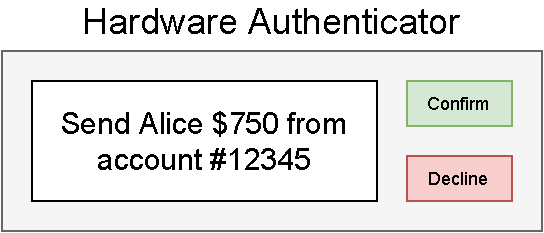
\includegraphics[width=10cm]{authenticator_drawio}
  \caption{User interface of hardware authenticator.}
  \label{Fig:HardwareAuthenticatorView}
\end{figure}

%% 
%% \iffalse
%% In the adversarial event that Alice were in fact malicious

%%  and the monetary transfer is actually intended for Bob

%% the user's web-browser were compromised and attempts to perform this unintended monetary transfer, 
%% \fi
%% 

This message contains enough information such that the user is fully informed of the operation they are about to perform. They can then make the educated judgment for whether to confirm the operation or not. In the adversarial event where a modified or unsolicited monetary transfer is attempted, the user should notice a discrepancy in the authentication message and decline the operation on the hardware authenticator. 

The goal of transaction authentication is to prevent the adversary from launching unsolicited operations on behalf of the user and causing fraudulence or damage. The operations that matter will require this additional authentication which the adversary cannot falsify as per the threat model --- the hardware device is assumed secure. This is a safe assumption because the hardware device is specialized to only perform this authentication process and nothing else. Ideally, it has a small attack surface that is vetted by security specialists. 

When the user authorizes this high-risk operation on their hardware authenticator, the message is cryptographically signed by the authenticator and sent back to the verifying end where it is checked. Only then, upon successful verification is the operation performed. 

Which operations should be protected is entirely at the discretion of the administrator of the web service. There is no clear-cut formula on what to protect, but candidate high-risk operations could include, but are not limited to, deleting one's account, transferring money, managing administrative permissions, publishing important software releases, etc. 


%% 
%% \iffalse

%% A security mechanism needs to protect against a stronger threat model in order to further harden a website's security. The threat model can be extended to where most of the transmission chain: the host computer, the operating system, web-browser, network and any other intermediate system may be compromised. And even under such a far-reaching threat model, the security mechanism must prevent unauthorized adversarial operation. What is assumed secure includes only the server code and hardware authenticator, as well as the entire registration event.

%% Traditional two-factor authentication may be simply extended as proposed by the WebAuthn specification \cite{TODO-WebAuthn} released by the World-Wide-Web Consortium (W3C) to work within this new and more restrictive threat model to defend against the class of vulnerabilities not covered by traditional two-factor authentication. This extension is called transaction authentication (txAuthn), and its goal is to enable "high-risk" operations to be individually authenticated by the user's hardware authenticator, despite the user being already logged in.

%% More specifically, when the user tries to issue some high-risk operation, they will be prompted with a message displayed on their paired hardware authenticator. The message is specific to the operation the user is trying to do, and should contain enough information needed for the user to verify that this is indeed the correct operation they want to perform. Upon acceptance by the user, the message is cryptographically signed by the hardware authenticator and sent back to the server where it gets verified, and only then, upon successful verification, is the operation performed.

%% A website, which assumes the more advanced threat model as described, would use transaction authentication to prevent any high-risk operations from being maliciously issued on behalf of the user. Such high-risk operations include, but are not limited to, deleting one's account, transferring money, managing administrative permissions, publishing important software releases, etc. 

%% For example, a bank website could require that monetary transfers exceeding \$500 must be transaction authenticated. In such a case, a possible authentication message that the user would have to confirm could resemble ``Send Alice \$750 from account \#12345''. This message contains enough information such that the user is fully informed as to what operation they are performing. Additionally, in the event that Alice is malicious and the transaction was actually intended for Bob, the user should notice this discrepancy in the authentication message and decline the operation on the hardware authenticator. 

%% \fi
%% 

%% 
%% \iffalse
%% The security benefits brought by transaction authentication to a web service would have a very tangible effect on the website's overall security. Client-side users of the application would have more faith that the website is operating correctly and not doing anything unauthorized at an adversary's request. Administrators of the website would rest more peacefully knowing that even if an adversary got access to their admin panel, they would not be able to do much damage as the critical operations require authentication from a physical hardware devices. And in general as a whole business, greater security would curb unnecessary losses due to hacker exploits and bolster greater trust in the general public's eye.
%% \fi
%% 

\section{Status Quo of Transaction Authentication}\label{Sec:StatusQuo}

%% 
%% \iffalse
%% Although transaction authentication is described in the WebAuthn protocol specification, no service or hardware authenticator has support for it. 
%% \fi
%% 

Although there are web services and hardware authenticators that support WebAuthn two-factor authentication, no service or authenticator supports the transaction authentication extension. Apart from transaction authentication not being integrated into real-world applications, there also has been no investigation into the implications of where it fits well, where it is inhibitory or unnecessary, what it takes to support transaction authentication in a web service and any software system designs that would help with integrating and configuring WebAuthn for an existing service.

%% 
%% \iffalse
%% In every case, there is what appears to be an almost standard practice for how WebAuthn gets used and integrated into a web service.
%% \fi
%% 

There are several publicly available codebases in the form of demo applets and libraries that work with WebAuthn transaction authentication~\cite{webauthn-online-examples} which illustrate how it can be used in a website. A website typically consists of a frontend and a backend. The frontend is the HTML/CSS/JavaScript that runs in the user's web-browser and is the origin of all of the user's requests when interacting with the website. The backend consists of the server code and database that execute the user's requests from the frontend. 

A web service using WebAuthn transaction authentication would have the frontend issue the WebAuthn requests and have the backend contain the WebAuthn library code to verify those requests and permit the operation if validation passes. Such approach to integrating WebAuthn has a number of practical downsides. 

%% 
%% \iffalse
%% Although this is a straightforward approach and is reasonable for a small applet web service, it begins to suffer when used on a larger codebase where the backend is complicated. 
%% \fi
%% 

Firstly, the backend architecture might not lend itself well to the control flow of the WebAuthn specification. In order to validate a WebAuthn request, multiple HTTP requests need to be sent back and forth between the frontend and backend. This may not be handled well by the backend if it was built under the assumption that there is only one HTTP request per operation.

Secondly, the integration of WebAuthn transaction authentication into a backend web service tends to be challenging for larger web services. The handler code for each operation is spread throughout the codebase, so it is difficult to keep track of what is secured and where in the code it is. Also, it requires a strong overall understanding of the web service code, which comes with its own set of challenges and slow development speed.

Lastly, in the extreme, albeit unlikely case, the backend may not even be accessible to the software developer if it is, for example, a closed-source API backend. In this case it is impossible to integrate WebAuthn into such a backend.

\section{Thesis Contributions}

There are three major contributions of this thesis:

\begin{enumerate}[nosep]

\item \sys{}: A firewall system design for integrating WebAuthn transaction authentication into a new or existing web service.

\item Three distinct case studies showcasing \sys{}. Each case study observes a class of web service and is used to test the limits of the usability of \sys{}.

\item A discussion on the beneficial use cases for transaction authentication, when it makes sense to be applied and when not.

\end{enumerate}

%% 
%% \iffalse
%% A second contribution is the use of the firewall in three distinct case studies.  The last contribution is a discussion on proper (and improper) usage of WebAuthn transaction authentication.
%% \fi
%% 

\subsection{WebAuthn Firewall}

Firstly, it must be emphasized that WebAuthn is simply a protocol specification. Implementation details are not bound to any one way, as long as they comply with the protocol's details. However, the code demos of WebAuthn unanimously integrate it into their codebases in the same intrusive manner. They import a WebAuthn library~\cite{webauthn-library} directly into the codebase and perform the necessary checks and validation in the backend.

\begin{figure}[h]
  \centering
  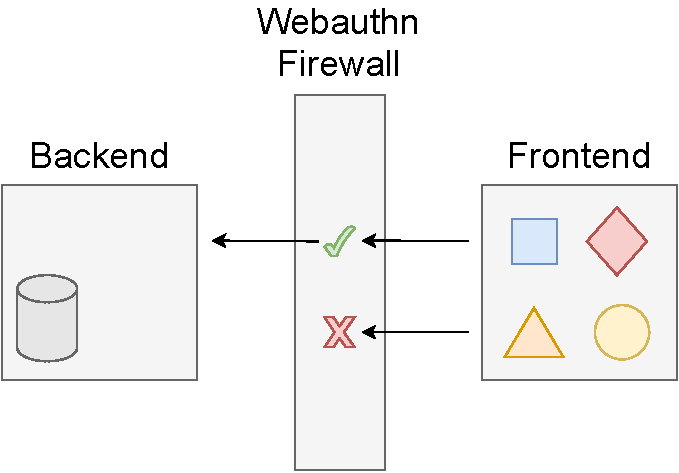
\includegraphics[width=12cm]{firewall_drawio}
  \caption{Basic depiction of the WebAuthn firewall functionality.}
  \label{Fig:BasicFirewallDepiction}
\end{figure}

This thesis proposes an alternative method for integrating WebAuthn by incorporating \sys{}, a Web Application Firewall (WAF). This firewall monitors and filters HTTP traffic sent from the website webpage to the backend. Any requests that the firewall deems as needing WebAuthn transaction authentication are stopped and processed by it. The firewall validates the request according to the WebAuthn transaction authentication specification. Figure~\ref{Fig:BasicFirewallDepiction} depicts how if the validation succeeds, then the firewall lets the request pass on through to the backend. If not, then the request is blocked. As far as the backend is concerned, it is unaware that \sys{} exists between it and the website webpage. 

With the WebAuthn firewall approach, the backend has to be minimally, if at all, modified to support WebAuthn transaction authentication. Although the frontend still needs to be modified to produce the WebAuthn transaction authentication requests as it is the origin of all of the user's operations, the firewall approach lends itself better to integrating WebAuthn into a new or existing web service. It is less intrusive than the traditional library-based approach and consolidates all of the WebAuthn related code in one place. As a result, it is less error-prone and easier to configure. 

%% 
%% \iffalse
%% . Needless to say, such a system design 
%% \fi
%% 

%% TODO: Is mentioning that the firewall is its own application, independent of the frontend or backend, worthwhile?

%% 
%% \iffalse
%% Additionally, the WebAuthn firewall is independent of the frontend and backend. 
%% \fi
%% 

The design of \sys{} presented in this thesis goes beyond simply providing a description and base functionality. It supplies the software engineer with useful defaults and a domain specific language (DSL) to configure \sys{}. Namely with a short configuration, the engineer can adapt \sys{} to parse and understand whatever input request format the web service uses. Requests map to operations in a web service depending on which HTTP route they are sent to. With only a few lines of code per route in the \sys{} configuration, the engineer can specify that the route be checked with transaction authentication and what the authentication message should be in order to pass as valid for that operation. 

%% 
%% \iffalse
%% The firewall handles the back-and-forth HTTP requests required for WebAuthn authentication. 

%% So it is much easier for the software engineer to organize and control what operations need transaction authentication and how exactly they get secured. 
%% \fi
%% 

%% 
%% \iffalse
%% % TODO: Are there demos for txAuthn or just WebAuthn. I think the latter only
%% Despite no major applications of WebAuthn, there are several publicly available codebases in the form of demo applets and libraries that work with WebAuthn \cite{TODO-WebAuthn-codebases-from-WebAuthn-website}. In every case, there is what appears to be an almost standard practice for how WebAuthn gets used and integrated into a service. A website typically consists of a frontend and a backend. The frontend is the web code that runs in the user's web-browser and is the origin of all of the user's requests when interacting with the website. The backend consists of the server code and database store that actually operates the website. Traditionally a web service using WebAuthn would have the frontend issue the WebAuthn requests and have the backend contain the code to verify those requests and permit the operation if everything passes. The principal contribution of this thesis demonstrates that there are alternative methods to using and integrating WebAuthn.
%% \fi
%% 

\subsection{Case Studies}

\begin{figure}[h]
  \centering
  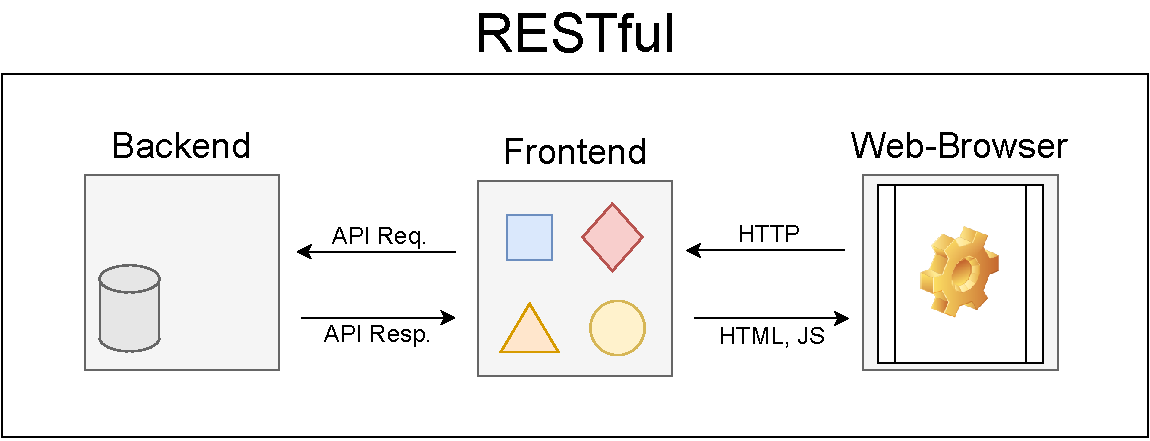
\includegraphics[width=10cm]{RESTful_drawio}
  \caption{The architecture design of a RESTful web application.}
  \label{Fig:CaseStudiesRESTful}
\end{figure}

\begin{figure}[h]
  \centering
  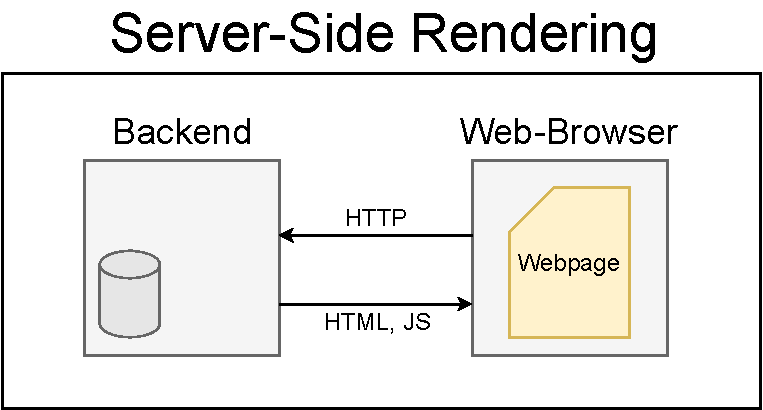
\includegraphics[width=9cm]{ServerSide_drawio}
  \caption{The architecture design of a server-side rendering web application.}
  \label{Fig:CaseStudiesServerSide}
\end{figure}

Three separate case studies demonstrate how \sys{} secures different architectures of web applications with WebAuthn transaction authentication. The web applications studied cover the RESTful design paradigm and the more traditional server-side rendering paradigm. The two RESTful applications studied are Conduit~\cite{conduit}, a simple blogging website, and Calypso~\cite{calypso}, a frontend admin panel for WordPress. As illustrated in Figure~\ref{Fig:CaseStudiesRESTful}, the RESTful paradigm is where the frontend runs in the web-browser separately from the web server backend program. The frontend performs the rendering visible to the user, and whenever it needs to fetch information or has to perform some server operation, it communicates via a pre-established API to the web server, which executes those requests. 

The server-side rendering application studied is Gogs~\cite{gogs}, a self-hosted Git service much like GitHub~\cite{github}. Figure~\ref{Fig:CaseStudiesServerSide} depicts the server-side rendering paradigm, where every operation the user performs on the webpage is sent over to the server as an HTTP request. In response, the server returns a whole new webpage, complete with all of the HTML and JavaScript code to be displayed on the user's web-browser.

%% 
%% \iffalse
%% . In return, everything that the user sees gets rendered on the server and is sent back as HTML code to be displayed directly by the user's web-browser.
%% \fi
%% 

These case studies stress test the flexibility and configurability of \sys{}. They are critical in establishing what parameters and configurable knobs \sys{} should provide. They are also used to evaluate how tangible the improvements are for using \sys{} in a web service rather than integrating WebAuthn transaction authentication intrusively. 

%% 
%% \iffalse
%% Lines of code, complexity, configurability, and integration difficulty are all evaluation criteria which support the use of the WebAuthn firewall over the traditional method.
%% \fi
%% 

\subsection{Other WebAuthn Possibilities}

In this thesis, Chapter~\ref{Chap:DiscussionAndFutureWork} gives insights into best practices relating to utilizing WebAuthn transaction authentication to secure various classes of problems. Researching transaction authentication reveals clear use cases where it lends itself well to secure, some use cases which are possible to secure, but not optimal, and lastly some use cases which cannot be protected at all by transaction authentication. 

%% 
%% \iffalse
%% There is future work that builds on from some of the insights provided by this research. web service routes can be analyzed to verify there is no way to subvert any protected routes. Also transaction authentication can be used to lessen how much code in the transmission chain must be trusted, to provide an even stricter threat model than the one assumed for the WebAuthn firewall. 
%% \fi
%% 

%% 
%% \iffalse
%% \subsection{WebAuthn Status Quo}

%% Firstly, it must be emphasized that WebAuthn is simply a protocol specification. Implementation details are not bound to any one way, as long as they comply with the protocol's details. However, the code demos of webauthn unanimously integrate it into their applet services in the same intrusive manner. They import a webauthn library in one of the many supported languages~\cite{TODO-webauthn-libraries} that performs the various validity and authentication checks along the webauthn specification. Then directly in the applications codebase, they invoke the library where it webauthn security is needed. This is a very straightforward coding practice and is very reasonable for a small applet web service. However, the same approach begins to suffer when used on a larger codebase when the backend is complicated and its architecture might not even lend itself well to the control flow of the webauthn specification. In order to validate a webauthn request, multiple HTTP requests need to be sent back and forth between the frontend and backend. This may not be handled well by the backend if it was built under the assumption that one HTTP request per operation. In other cases, the backend is fully inaccessible because it is part of a closed-source software project. 

%% \subsection{Overview of Contributions}

%% An alternative method for integrating webauthn is as a Web Application Firewall (WAF). This firewall monitors and filters HTTP traffic sent from the frontend to the backend. Any requests that the firewall deems as needing further webauthn transaction authentication get stopped. The firewall handles the back-and-forth HTTP requests required for webauthn authentication. And if all succeeds, it lets the request pass on through to the backend. As far as the backend is concerned, it is virtually unaware that a firewall exists between it and the frontend performing the webauthn validation. Under such webauthn firewall approach, the backend has to be minimally, if at all, modified to support webauthn transaction authentication. The frontend still needs to be modified to produce the webauthn transaction authentication requests as it is the origin of all of the user's operations. Needless to say, such a system design lends itself much better for integrating webauthn into a new or existing web service. It is much less intrusive than the traditional library-based method. As a result, it is much less error-prone and easier to configure. Additionally, the webauthn firewall is independent of the frontend and backend. So it is much easier for the software engineer to organize and control what operations need transaction authentication and how exactly they get secured. 

%% The webauthn firewall presented in this thesis goes beyond simply providing base functionality. It supplies the software engineer with useful defaults and a powerful domain specific language (DSL) to configure the firewall. Namely with a short configuration, the engineer can adapt the firewall to parse and understand whatever input request format the web service uses. Additionally, with only a few lines of code per HTTP route, they can also specify that the route gets checked with transaction authentication and what the authentication message should be in order to pass as valid for that operation. 

%% Furthermore, case studies demonstrate how the webauthn firewall secures three different architectures of web applications with webauthn transaction authentication. The web applications studied cover the RESTful design paradigm and the more traditional server-side rendering paradigm. The RESTful paradigm is where the webpage frontend and web-server backend are two separate programs. The frontend performs the rendering visible to the user, and whenever it needs to fetch information or has to perform some server operation, it communicates via a standardized API to the web-server which executes those requests. The server-side rendering paradigm is where every operation the user performs on the webpage gets requested to the server directly. In return, everything that the user sees gets rendered on the server and is sent back as HTML code to be displayed directly by the user's web-browser.

%% These case studies stress test the flexibility and configurability of the webauthn firewall. They were critical in establishing what parameters and configurable knobs the firewall should provide. They are also used to evaluate how tangible the improvements are for using the firewall in a service rather than more traditionally integrating webauthn transaction authentication intrusively. Lines of code, complexity, configurability, and integration difficulty are all evaluation criteria which support the use of the webauthn firewall over the traditional method.

%% Beyond describing the webauthn firewall, the thesis will also give insights into best practices relating to utilizing webauthn transaction authentication to secure various classes of problems. Researching transaction authentication revealed clear use cases where it lends itself well to secure, some use cases which are doable to secure, but not optimal, and lastly some use cases which are not protected at all be transaction authentication. There is future work that builds on from some of the insights provided by this research. web service routes can be analyzed to verify there is no way to subvert any protected routes. Also transaction authentication can be used to lessen how much code in the transmission chain must be trusted, to provide an even stricter threat model than the one assumed for the webauthn firewall. 
%% \fi
%% 

%% 
%% \iffalse
%% in order a protected operation to be processed by the web-server, it must be 

%% but it is not void of vulnerabilities

%% with only a few lines of code per HTTP route, the engineer can adapt the firewall to parse and understand whatever input request format the web service uses. 

%% specify whether the route gets checked with transaction authentication and what the authentication message should be to pass as valid for that operation. 

%% Each  how well it can support a variety of different web applications, each with different 
%% \fi
%% 

\subsection{Source Code}

The source code of \sys{} and case studies is publicly available at \url{https://github.com/JSmith-BitFlipper/Guarda-firewall} under the MIT License.

%% 
%% \iffalse
%% Cheers! 
%% \fi
%% 

\section{Thesis Outline}

The thesis contains the following chapters. Chapter~\ref{Chap:RelatedWork} discusses the related work and background pertinent to this research. Chapter~\ref{Chap:WebauthnTransactionAuthentication} describes the WebAuthn transaction authentication protocol in detail. Chapter~\ref{Chap:WebauthnFirewallDesign} outlines the design of \sys{}, the WebAuthn firewall. Chapter~\ref{Chap:WebauthnFirewallImplementation} discusses the implementation details of the novel components of \sys{}. Chapter~\ref{Chap:CaseStudies} explains the case studies of \sys{}. Chapter~\ref{Chap:Evaluation} contains the experiments and evaluation metrics for \sys{}. Chapter~\ref{Chap:DiscussionAndFutureWork} opens a discussion of supplemental notes uncovered over the course of this research. Finally, Chapter~\ref{Chap:Conclusion} concludes this thesis.

%% This is an example first chapter.  You should put chapter/appendix that you
%% write into a separate file, and add a line \include{yourfilename} to
%% main.tex, where `yourfilename.tex' is the name of the chapter/appendix file.
%% You can process specific files by typing their names in at the 
%% \files=
%% prompt when you run the file main.tex through LaTeX.
\chapter{Related Work}\label{Chap:RelatedWork}

This chapter presents the background and related work that precedes this research. These concepts lay out the foundation on which the rest of this research is conducted.

% TODO: Maybe explain what external observation and internal observation are
\section{Hardware Authenticators for \newline Two-Factor Authentication}\label{Sec:HardwareAuthenticators_2FA}

The state of the art for using hardware devices for website authentication is two-factor authentication. These devices such as the YubiKey \cite{yubico-products} resemble a small USB key which stores a private key on device. Websites that support two-factor authentication simply request the secondary mode of authentication during login. Two-factor authentication solves the security problems for login quite well \cite{questRemovePasswords}. Depending on the implementation of the specific hardware device, most provide strong resilience to targeted impersonation, physical observation, internal observation, leakage of data secrets and relying on a trusted third-party. However, as explained previously, these benefits do not pertain beyond the login point of a website and assume a lenient threat model. The adversary with control over the web-browser could simply wait for the user to faithfully log in and then launch their planned attack. 

%% 
%% \iffalse
%% , in addition to supplying a password. 
%% \fi
%% 

A number of specifications standardize two-factor authentication so that the same hardware authenticator device may be used across platforms and web services. A popular standard is Universal 2nd Factor (U2F) \cite{fido-u2f} developed by Google and Yubico, now hosted by the open-authentication industry consortium FIDO (``Fast IDentity Online'') Alliance. It is succeeded by FIDO2 \cite{fido2}, which merges WebAuthn and its extensions, including transaction authentication, into one common standard.

\section{Current Uses of Transaction Authentication}\label{Sec:CurrentUses_txAuthn}

Although transaction authentication by the WebAuthn standard is not yet commonly used, cryptocurrency hardware wallets universally support transaction authentication. The two most popular manufacturers, Ledger \cite{ledger} and Trezor \cite{trezor}, sell hardware wallets which hold the private keys and have displays. In order to send any cryptocurrency from the device, the device displays a message detailing the transaction, which the user would need to authorize on the physical device. Otherwise, the device will not sign the transaction which is required for it to proceed and be sent over the network.

In a similar but diminished vain, some banks such as Bank of America reuse two-factor authentication for sensitive or high-value monetary transactions \cite{BoA-2FA}. In order to complete the sensitive transaction, the user must redo two-factor authentication like during login. This is unlike transaction authentication in that no hardware device specific to transaction authentication is involved, and the user does not see a confirmation of the exact transaction to take place before confirming. But the process of requesting supplemental two-factor authentication on sensitive transactions aims to defend against a similar threat model as transaction authentication.

\section{Hardware Authenticators for \newline Transaction Authentication}

Hardware authenticator devices normally do not support general-purpose transaction authentication. Hardware authenticators for two-factor authentication such as the YubiKey discussed in Section~\ref{Sec:HardwareAuthenticators_2FA} do not have any display. Therefore, they are unable to perform the core function of transaction authentication, displaying a message to the user and signing it upon their confirmation. The cryptocurrency hardware wallets discussed in Section~\ref{Sec:CurrentUses_txAuthn} provide transaction authentication, but only for a limited subset of functionality relating to crypto transactions.  

%% 
\iffalse
, but none support the transaction authentication extension.

are dedicated hardware devices required by the threat model. Also, these authenticators only support regular WebAuthn two-factor authentication, not the transaction authentication extension. 
\fi
%% 

WebAuthn transaction authentication is not supported by any hardware authenticators. A few hardware authenticators and software emulated authenticators support WebAuthn, but only the regular two-factor authentication. The software emulated authenticators are intended for development and research purposes. Google has a Chrome extension that poses as a virtual hardware authenticator; it performs all of the signing in-browser \cite{virtual-authenticators-tab}. Krypton is a small company dedicated to making cryptographic authentication easy \cite{krypton}. They provide a browser plugin and phone app, which pair with one another. The plugin interfaces with the web-browser and the phone performs the cryptographic signing. 

This research must modify one of the software emulated authenticators to support transaction authentication. It uses a modified Krypton browser plugin to display the authentication message and await user consent before performing the signing also in-browser. Figure~\ref{Fig:KryptonAuthenticator} portrays the user interface of the plugin as it awaits consent before returning a signed transaction authentication object. This design deviates from the original Krypton design since it eliminates the phone app from the signing process. The security properties of the authenticator device itself is not a focus for this research. It is assumed always secure, so for prototyping and experimentation, this software modified authenticator is sufficient.

\begin{figure}[h]
  \centering
  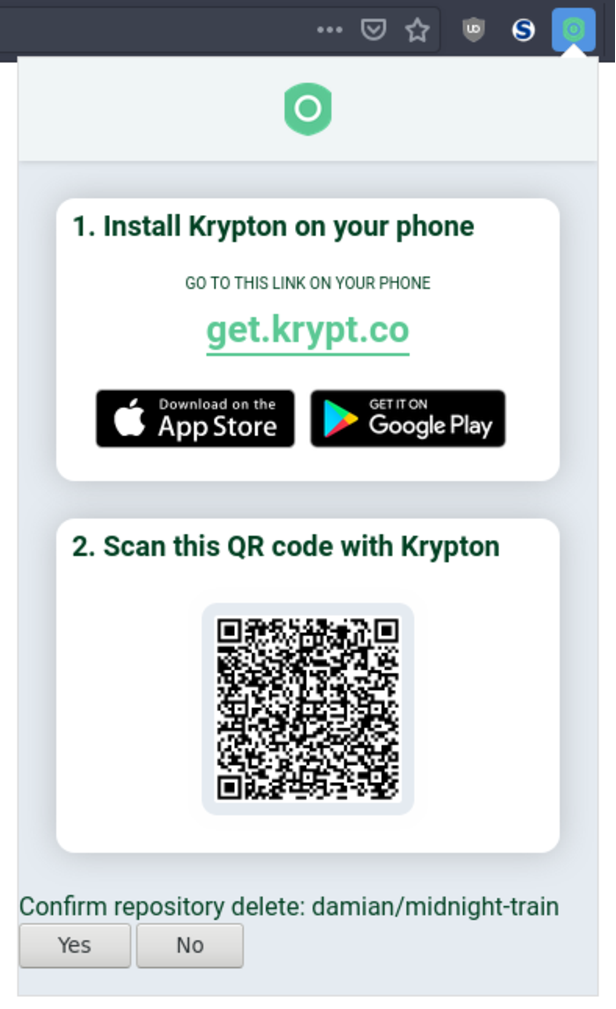
\includegraphics[width=10cm]{krypton_txauthn}
  \caption{User interface of Krypton authenticator in this thesis. It is awaiting user consent before authorizing the deletion of a repository ``damian/midnight-train''.}
  \label{Fig:KryptonAuthenticator}
\end{figure}

%% 
%% \iffalse
%% For ease of development, this research modified the Krypton browser plugin to display the authentication message and await user consent before performing the signing in-browser. It completely

%% Since the design of the hardware authenticator is not a focus for this research, it is simpler to avoid interfacing with the phone at all. 
%% \fi
%% 

\section{Web Application Firewalls}

A Web Application Firewall is a firewall that filters web traffic going to a web service \cite{web-application-firewall}. Most web application firewalls try to block malicious internet traffic from ever reaching the web server. Common attacks defended against by web application firewalls include SQL injection, cross-site scripting and DDoS attacks. Typically, the firewall inspects incoming GET and POST request HTTP/HTTPS traffic and applies pre-configured rules to identify and filter out the undesired traffic. This thesis describes how to make a web application firewall supporting WebAuthn transaction authentication.


%% 
%% \iffalse

%% This research builds on top of the description of transaction authentication as outlined by the first version of the webauthn specification \cite{webauthn}. The webauthn specification is a comprehensive document, standardizing a protocol for two-factor authentication with configurable extensions. The protocol covers in detail how traditional two-factor authentication should be performed under webauthn as well as details how to extend it to perform transaction authentication. Transaction authentication is similar to a regular two-factor authentication event, just with some additional user involvement; the user must confirm a given transaction on a dedicated hardware device for the authentication to proceed. 

%% The purpose of transaction authentication in the eyes of the webauthn specification authors is to provide integrity to high risk operations on a website. In fact, further papers including \cite{EuroFIDO} detail use-cases of webauthn transaction authentication such as authorizing large value monetary transactions, consenting to data being shared with a third-party and authorizing a trusted service to sign a digital contract. All of these operations are very important and requesting individual authentication for each may be warranted. 

%% It appears that the state of the art for known security benefits through transaction authentication ends there. There is no research detailing how webauthn transaction authentication should be integrated into a service, what are good design choices in doing so or what the engineer should keep in mind in order to avoid accidental security holes.

%% \fi
%% 

%% This is an example first chapter.  You should put chapter/appendix that you
%% write into a separate file, and add a line \include{yourfilename} to
%% main.tex, where `yourfilename.tex' is the name of the chapter/appendix file.
%% You can process specific files by typing their names in at the 
%% \files=
%% prompt when you run the file main.tex through LaTeX.
\chapter{Webauthn Transaction Authentication}\label{Chap:WebauthnTransactionAuthentication}

Webauthn transaction authentication is a protocol specification for authenticating high-risk user operations, even after login. The specification describes a sequence of steps that must be followed in order to authenticate properly. These steps can be split into four stages, registration, the setup, the cryptographic attestation and then the verification. 

\begin{enumerate}[nosep]
\item Registration: Makes a record of the user and their cryptographic credential into a database store later accessible to the verification code and is performed only once per user.

\item Setup: Initiated by the user's web-browser and involves a priming exchange between it and the webauthn verification end.

\item Cryptographic Attestation: Occurs on the hardware authenticator device after the user confirms the operation. The threat model assumes that this attestation is always secure.

\item Verification: Validates whether to authorize the high-risk user operation or not. Checks if the requested operation matches its authentication message and that the cryptographic signature on it is valid. This stage also is assumed secure under the threat model.

\end{enumerate}

This outline for transaction authentication uses the webauthn firewall as the verification end. It contains the database of user public key credentials and performs the validation to authorize high-risk operations or not. As webauthn is a protocol specification, nothing dictates this design choice. However, for continuity with the thesis work, the protocol is best explained with the firewall.

%% 
%% \iffalse
%% between the user and hardware authenticator device. 

%% Lastly, the verification stage 
%% Occurs within the firewall, and it 
%% \fi
%% 

\subsection{Webauthn Registration}

\begin{center}
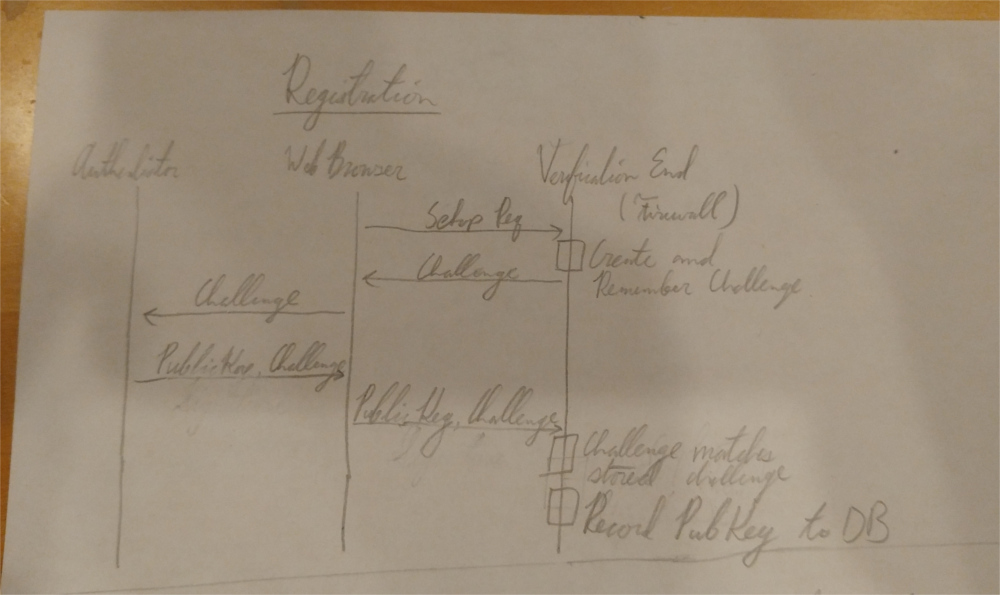
\includegraphics[width=12cm]{registration_flow}
\end{center}

During the registration event, the user's hardware device sends its public key credential to the firewall. This process is completely secure in the threat model, with no adversary to intercept or tamper with any of the communication. Therefore, whatever credential the firewall receives during registration is assumed to be genuine and the user's. The firewall later on uses this credential during the verification stage to ensure transaction authentication integrity. The registration process begins with a setup of its own, where the web-browser requests a few parameters from the firewall, most notably a random challenge nonce.

%% 
%% \iffalse
%% \begin{lstlisting}
%% type PublicKeyCredentialCreationOptions struct {
%% 	Challenge              Challenge                
%% 	RelyingParty           RelyingPartyEntity       
%% 	User                   UserEntity               
%% 	Parameters             []CredentialParameter
%% 	AuthenticatorSelection AuthenticatorSelection
%% 	Timeout                int                      
%% 	Attestation            ConveyancePreference
%% }
%% \end{lstlisting}
%% \fi
%% 

The firewall remembers the challenge it sent as a part of the session data associated with the registration setup request. The challenge nonce prevents replay attacks \cite{TODO-replay-attack}. There are a few other parameters, but they are mainly for the hardware device to know what type of credential the firewall is expecting to receive. The hardware device sends over its public key credential for the firewall to save, with the challenge signed by that credential. The firewall receives an HTTP POST request containing this public key credential. The POST request also contains identifying information of the current user. The firewall verifies that the challenge is matches, and upon success, stores the credential and associated user ID into a database row.

\subsection{Transaction Authentication Setup}\label{Sec:TransactionAuthenticationSetup}

\begin{center}
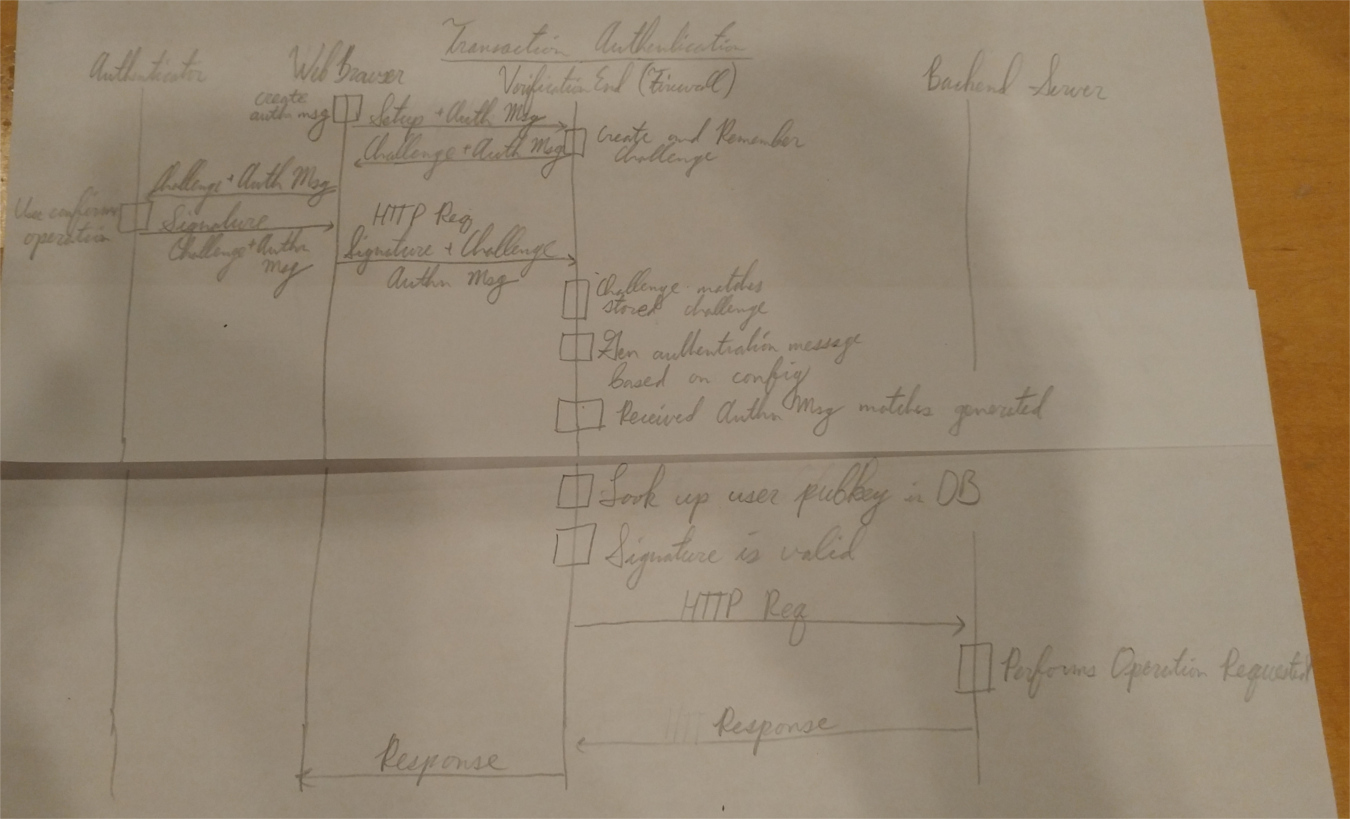
\includegraphics[width=15cm]{txauthn_flow}
\end{center}

% TODO: Talk about server-side rendering preloading

The setup for a transaction authenticate event generally originates from the frontend. There are several designs to setup a webauthn transaction event, but the setup content itself is all the same. More commonly, setup may occur lazily where the frontend waits for the user to initiate an operation protected by transaction authentication before initiating the setup. Or it may occur eagerly where the frontend preemptively initiates the setup, without knowing whether the user will even perform any secured operation on the web-page. Nonetheless, the setup is a POST request to the firewall. The payload for the setup POST request is an authentication message that will eventually be displayed to the user on their hardware device. The message is constructed from any user input and any additional information contained in the HTML of the webpage, but in all three case studies of this thesis, that was always enough. In response, the frontend receives a few parameters:

%% 
%% \iffalse
%% \begin{lstlisting}
%% type PublicKeyCredentialRequestOptions struct {
%% 	Challenge          Challenge                   
%% 	Timeout            int                         
%% 	RelyingPartyID     string                      
%% 	AllowedCredentials []CredentialDescriptor      
%% 	UserVerification   UserVerificationRequirement 
%% 	Extensions         AuthenticationExtensions    
%% }
%% \end{lstlisting}
%% \fi
%% 

Most importantly, a random \lstinline{challenge} nonce is returned. The firewall remembers it locally in the session data associated with the request. When the firewall processes the protected request, it will verify that the challenge included in the returned authentication data matches the one previously sent and remembered in the session. An adversary cannot intercept and replay old protected requests since it is exceedingly unlikely that future challenges from the firewall will exactly match the challenge in the intercepted request. 

An \lstinline{extensions} field is also returned, following the webauthn protocol. The firewall took the authentication message sent to it and transformed it into a form which any webauthn-compatible hardware authenticator should handle as a transaction authentication operation.

%% 
%% \iffalse
%% There are other fields returned as a part of the setup, but they are mostly for plumbing. They delineate how the hardware device should respond when authenticating the webauthn transaction.
%% \fi
%% 

%% 
%% \iffalse
%% The other fields are mostly for plumbing. The \lstinline{Timeout} requires an authentication response with that amount of time. The \lstinline{RelyingPartyID} identifies the backend. The \lstinline{AllowedCredentials} identifies with which cryptographic key the user can sign the response. The \lstinline{UserVerification} tells the hardware authenticator that the user must physically confirm ``yes'' or deny ``no'' a request and is usually set to \lstinline{true}. The \lstinline{Extensions} includes a signal that transaction authentication is to be performed with the authentication message sent to the firewall.
%% \fi
%% 

\subsection{Cryptographic Attestation}\label{Sec:CryptographicAttestation}

The request options from the firewall go through the frontend and are passed on to the hardware authenticator device. The threat model assumes that only the firewall, backend and hardware authenticator are secure. At any point, the frontend or web-browser could modify these options, but any tampering will be detected later on and denied authorization. The hardware device parses the request options, extracts from the \lstinline{extensions} field the authentication message and presents that to the user. The authentication message is in the form of a confirmation for some requested operation and is answered either by ``yes'' or ``no''. If the user attests ``yes'', the hardware device cryptographically signs a data object which is returned as an additional field within the HTTP request to the firewall for verification.

The response of the hardware authenticator includes a \lstinline{clientDataJSON} object containing the authentication message displayed to the user a well as the \lstinline{Challenge} from the setup stage. A cryptographic signature of the \lstinline{clientDataJSON} is also included. Specifically, Elliptic Curve Digital Signature Algorithm (ECDSA) paired with the SHA-256 hash function is the signing function. There are other fields, as well, for plumbing to help the firewall know what parameters to use to validate this response.

%% 
%% \iffalse
%% % TODO: Make this typescript highlighting
%% \begin{lstlisting}
%% const credential: PublicKeyCredential = {
%%     id: string, // base64 encoded
%%     rawId: []bytes,
%%     response: {
%%         attestationObject: []bytes,
%%         clientDataJSON: {
%%             challenge: string, // base64 encoded
%%             clientExtensions: []bytes,
%%             hashAlgorithm: string,
%%             origin: string,
%%         },
%%     },
%%     type: 'public-key',
%% };
%% \end{lstlisting}

%% The \lstinline{clientDataJSON} contains the \lstinline{clientExtensions} which is the data displayed to the user as well as the \lstinline{challenge} from the setup stage. The cryptographic signature of the \lstinline{clientDataJSON} is included in the \lstinline{attestationObject} and uses the Elliptic Curve Digital Signature Algorithm (ECDSA) paired with the SHA-256 hash function. The other fields are for plumbing and help the firewall know what parameters to use to validate this authentication data object.
%% \fi
%% 

\subsection{Webauthn Firewall Verification}\label{Sec:WebauthnFirewallVerification}

The webauthn firewall receives an HTTP request on a protected route with all of its usual parameters plus the authentication data object. The firewall must verify the integrity of this object as well that it corresponds with the intent of the HTTP request. In other words, it must detect whether any code not in the trusted computing base, such as the frontend, tampered with the authentication data. Also, it must make sure that the operation the user attested to on their hardware device that resulted in this authentication data object is in fact the operation to be performed if the protected HTTP request were to be permitted through. The three main steps of this verification are checking the challenge, the authentication message and the authentication data signature.

Checking the challenge is a simple comparison between the challenge received \lstinline{challenge} and the \lstinline{storedChallenge} in the firewall's session data. This protects against replay attacks.

%% 
%% \iffalse
%% \begin{lstlisting}
%% // Verify the challenge
%% Challenge := c.ClientDataJSON.Challenge
%% if strings.Compare(storedChallenge, Challenge) != 0 {
%% 	err := ErrVerification.WithDetails("Error validating challenge")
%% 	return err
%% }
%% \end{lstlisting}
%% \fi
%% 

Checking the authentication message is slightly more involved. The firewall is configured per route how to generate an expected authentication message based on the HTTP request parameters. This generated authentication message must unambiguously encapsulate the entire intent of the request. Details are further discussed in Section~\ref{Sec:AuthenticationMessage}. Then it is a simple comparison between the received \lstinline{clientMessage} and the \lstinline{generatedMessage}. This makes sure the user authenticated a message that faithfully represents the intent of the HTTP request.

%% 
%% \iffalse
%% \begin{lstlisting}
%% // Verify the authentication message
%% clientMessage := c.ClientDataJSON.Extensions["txAuthnSimple"]
%% if strings.Compare(generatedMessage, clientMessage) != 0 {
%% 	err := ErrVerification.WithDetails(
%%               "Error validating authentication message")
%% 	return err
%% }
%% \end{lstlisting}
%% \fi
%% 

Lastly, checking the authenticating data signature involves invoking cryptography library utilities. This validates the integrity of the entire authentication object to prove that it was not tampered with. The \lstinline{clientDataJSON} was signed by the hardware authenticator. The firewall has the public key of the hardware authenticator, so it can see if the \lstinline{clientDataJSON} indeed corresponds to the signature attributed to it.

%% 
%% \iffalse
%% \begin{lstlisting}
%% // Verify the signature

%% // The data signed by the hardware authenticator
%% clientDataHash := sha256.Sum256(c.ClientDataJSON)
%% sigData := append(p.Raw.AssertionResponse.AuthenticatorData, 
%%                   clientDataHash[:]...)

%% // The user's public key stored in the firewall
%% key, err := webauthncose.ParsePublicKey(credentialBytes)
%% valid, err := webauthncose.VerifySignature(
%%                  key, sigData, p.Response.Signature)
%% if !valid {
%% 	return err
%% }
%% \end{lstlisting}

%% Setup can occur eagerly where the web-browser immediately performs the setup without the user initiating any operation protected by transaction authentication.

%% If not, it will deny the request from continuing through.

%% The frontend only has access to the information it displays in the HTML to the user, 

%% The data displayed to the user along with its respective signature is included in the \lstinline{response} field. The hardware device signs
%% \fi
%% 

%% This is an example first chapter.  You should put chapter/appendix that you
%% write into a separate file, and add a line \include{yourfilename} to
%% main.tex, where `yourfilename.tex' is the name of the chapter/appendix file.
%% You can process specific files by typing their names in at the 
%% \files=
%% prompt when you run the file main.tex through LaTeX.
\chapter{Webauthn Firewall Design}

The webauthn firewall acts as a Web Application Firewall (WAF). It is situated directly between the frontend and backend, processing all user requests sent between the two. Each requests gets parsed by the firewall, and understood whether it is a request that needs webauthn transaction authentication or not. If not, the request is simply proxied through to the backend without any extra work. However, if it needs transaction authentication, the firewall as a gatekeeper for that request. The firewall performs a verification procedure on the request and only upon success does the request pass through the firewall to the backend. If it fails, the firewall returns an error back to the frontend. This design strategy for integrating webauthn transaction authentication into a service is very powerful because it is web service agnostic. The backend is completely unaware that the requests it receives are webauthn authenticated. Of course, since the frontend has to interface with the user's hardware authenticator device, it must be aware of webauthn, but only to a minor extent. 

\subsection{Proxying Requests}

In multiple case studies, the firewall was used to integrate webauthn transaction authentication into two different paradigms of web service designs, RESTful and server-side rendered websites. For each, the notion of the firewall being situated between the frontend and backend is slightly different, but the function and role of the webauthn firewall is the same, filtering, verifying and proxying requests. For a RESTful web application, the placement of the firewall is more intuitive. In a RESTful design, frontend and backend are separate programs running on their own IP addresses and ports. The user's web-browser interacts with the frontend through its IP address. And whenever the frontend needs to interact with the backend, it launches HTTP requests to the IP address of the backend. In a RESTful web service design, the webauthn firewall naturally sits in between the two. The firewall runs on its own IP address and port, and the frontend is reconfigured to use it as its backend address destination. So when the frontend needs to issue a backend request, it sends it rather to firewall rather than the backend. From there, the firewall performs its role and, as necessary, proxies onward to the actual backend. Responses from the backend are returned to the firewall which automatically get forwarded on to the frontend. In a server-side rendering web application, the firewall additionally performs the role of the frontend described in the RESTful use case. That is, the user's web-browser interacts with the IP address of the firewall directly. All HTTP requests originate from the user's web-browser and are directed to whatever the address is of the frontend. In a server-side rendering web application, the whole service, the frontend and backend, is served out of the same address. With the webauthn firewall, requests get sent to the firewall which again does its role and, if necessary, relays onward to the server-side rendering web-application. In this case, the webauthn firewall is situated between the web-browser and backend. But nonetheless, it is the same principle as with the RESTful web application use case. An origin, in this case the web-browser, issues requests destined for a backend, but they get intercepted by the firewall, before they continue on if everything succeeds.

\subsection{Webauthn Verification}

% TODO: Make option in firewall to either pass through or block non-specified requests. Modify this paragraph
% TODO: Explain basic webauthn txAuthn ecosystem

As the webauthn firewall filters requests sent to it, some requests will be held back to be webauthn transaction authenticated first. Which requests get held back and how they get verified is configured in the firewall by the software engineer. In order to specify which HTTP route to filter out and transaction authenticated, the engineer simply includes the route in the firewall's configuration. All other routes not specified in the configuration are simply passed on through to the backend without any checks.

\subsubsection{Authentication Message}

Of the requests that need to be checked, the engineer must specify how they get verified. In essence, verifying an incoming HTTP request with transaction authentication involves the firewall generating an authentication message from the parameters of the request. Then the verification passes only if the generated message is exactly identical to the message signed by the hardware authenticator also included in the request and the associated signature is valid. The message generated by the firewall represents the root of truth and should encapsulate the entire intent of the request in order to have good security guarantees. All of the parameters in the requests that are considered security sensitive must appear unambiguously in the authentication message in a human readable format. Unambiguity refers to how no two different requests can share the same authentication message. Human readability is critical since the user is the one authenticating the message and sometimes the parameters in the request may be not human intelligible such as object IDs, etc.

\subsubsection{Context Retrieval}

% TODO gets context

Where the HTTP request contains not human friendly identifiers that need to be understood by the user, those identifiers must be translated to their human readable counterparts. For example, an ID may identify some object in a web service. The firewall must generate...

\iffalse
is reconfigured to issue backend requests to the IP address

Upon opening the web page, requests are issued from the web-browser

has two options to specify how a route gets verified.

This message should encapsulate 
\fi

%% This is an example first chapter.  You should put chapter/appendix that you
%% write into a separate file, and add a line \include{yourfilename} to
%% main.tex, where `yourfilename.tex' is the name of the chapter/appendix file.
%% You can process specific files by typing their names in at the 
%% \files=
%% prompt when you run the file main.tex through LaTeX.

%% Topics:
%% Frontend modifications
%% Backend modifications
%% Implementation overview of default handlers 
%% Implementation of DSL and Authn function
%%   How this plays with:
%%   - default input getters
%%   - context retrieval 

\chapter{WebAuthn Firewall Implementation}\label{Chap:WebauthnFirewallImplementation}

The WebAuthn firewall studied is implemented in the Go programming language. This chapter describes how some of the critical components of the firewall's design detailed in Chapter~\ref{Chap:WebauthnFirewallDesign} are implemented. The following Table~\ref{Table:ImplementationFootprint} outlines the approximate footprint of each component discussed in this chapter.

\begin{table}[h]
\centering

\begin{tabular}{ m{5cm} m{3cm}  } 
 \hline
 Firewall Component & Lines of Code \\ 
 \hline \hline

 WebAuthn Verification & 126 \\ \hline

 Default Handlers & 309 \\ \hline

 Domain Specific Language & 478 \\ \hline

\end{tabular}
\caption{The domain specific language \lstinline{Get} type operations. These affect the format string if invoked at the top level within \lstinline|Authn|.}
\label{Table:ImplementationFootprint}
\end{table}

%% 
%% \iffalse
%% \section{Webauthn JavaScript Library}

%% The webauthn JavaScript library provides easy access to the webauthn setup and verification life-cycle for the frontend. It exposes a few functions which take care of the boilerplate code. 

%% The functions for setup are:

%% \begin{lstlisting}
%% const retrieveWebauthnOptions_FormField = async (form_id, field_name) => { ... }
%% const retrieveWebauthnOptions_Cookie = async (src_cookie) => { ... }
%% const retrieveWebauthnOptions_URL = async (form_id, src_url) => { ... }
%% \end{lstlisting}

%% They all access the setup data from the firewall by their respective payload types. The \lstinline{FormField} reads the data from a form in the current HTML page. The \lstinline{Cookie} reads the data from some cookie. And the most commonly used \lstinline{URL} performs a POST request and reads the setup data from the response.

%% The functions for registration are:

%% \begin{lstlisting}
%% const registrationFinish_URL = async (credentialCreateOptionsFromServer, finish_url, form_id) => { ... }
%% const registrationFinish_PostFn = async (credentialCreateOptionsFromServer, post_fn) => { ... }
%% \end{lstlisting}

%% They send over the hardware authenticator's credentials to the firewall during the registration event after the setup has been performed. Each performs the same processing procedure on the \lstinline{credentialCreateOptionsFromServer} webauthn options before issuing a POST request over to the firewall. The functions take the \lstinline{credentialCreateOptionsFromServer}, manipulate the encoding, get the hardware authenticator's credential and then package it into a clean JavaScript object. Fetching the hardware authenticator's credential is done with the web-browser exposing an API. The web-browser handles the interaction with the hardware device.

%% \begin{lstlisting}
%% const credential = await navigator.credentials.create({
%%   publicKey: publicKeyCredentialCreateOptions
%% });
%% \end{lstlisting}

%% The \lstinline{PostFn} function lets the caller specify a function, \lstinline{post_fn}, which performs the POST request instead of from the library as is the case with the \lstinline(URL) function.

%% The functions for webauthn transaction authentication:

%% \begin{lstlisting}
%% const attestationFinish_URL = async (credentialRequestOptionsFromServer, finish_url, form_id) => { ... }
%% const attestationFinish_PostFn = async (credentialRequestOptionsFromServer, post_fn) => { ... }
%% \end{lstlisting}

%% These functions are implemented nearly identically as their registration counterparts. The \lstinline{PostFn} function relies on a supplied \lstinline{post_fn} to issue the POST request whereas the \lstinline{URL} does it as a part of the library code. The primary difference is that the web-browser's API call is different.

%% \begin{lstlisting}
%% const assertion = await navigator.credentials.get({
%%     publicKey: transformedCredentialRequestOptions,
%% });
%% \end{lstlisting}

%% The \lstinline{transformedCredentialRequestOptions} contains all of the necessary transaction authentication setup information described in Section~\ref{Sec:TransactionAuthenticationSetup}, such as the challenge and the authentication message. This web-browser API call passes on that information to the hardware authenticator device. If the user confirms the operation on the hardware device, an \lstinline{assertion} is returned with the authentication data described in Section~\ref{Sec:WebauthnFirewallVerification}.
%% \fi
%% 

\section{WebAuthn Verification}\label{Sec:WebauthnVerification}

The cryptographic verification of a WebAuthn transaction authentication event uses a slightly modified Go WebAuthn library \cite{TODO-Golang-Webauthn-Library}. This library exposes two functions, \lstinline{BeginLogin} and \lstinline{FinishLogin}, which set up and validate a WebAuthn two-factor authentication event respectively. The \lstinline{FinishLogin} function is modified to support the transaction authentication extension. It checks if the extensions object received from the hardware authenticator exactly match an expected extensions object generated by the firewall.

%% 
%% \iffalse
%% The \lstinline{BeginLogin} call is invoked during the webauthn setup stage and is used straightforwardly.

%% \begin{lstlisting}
%% // Generate the webauthn `options` and `sessionData`
%% options, sessionData, err := webauthnAPI.BeginLogin(wuser)
%% if r.HandleError(w, err) {
%%   return
%% }

%% \end{lstlisting}

%% The \lstinline{wuser} is a webauthn user entry from the firewall's database store. It contains typical information such as the user's ID and public key credential. Returned are the \lstinline{options} that get sent back to the frontend and eventually the hardware authenticator as the result of the setup stage. The \lstinline{sessionData} is remembered by the firewall for the current HTTP request as described in Section~\ref{Sec:TransactionAuthenticationSetup}.

%% The \lstinline{FinishLogin} call is invoked more selectively. If a user does not have webauthn currently enabled, that is they do not have a registered hardware device with the web service, then routes that are webauthn protected should not check for webauthn for that user's requests. The following is a simplification of the webauthn transaction verifying code.

%% \begin{lstlisting}
%% // See if the user has webauthn enabled
%% isEnabled := db.WebauthnStore.IsUserEnabled(db.QueryByUserID(userID))

%% // Perform a webauthn check if webauthn is enabled for this user
%% if isEnabled {
%%   // Parse the form-data to retrieve the `http.Request` information
%%   assertion, err := r.Get_WithErr("assertion")

%%   // Get the `authnText` to verify against
%%   authnText := getAuthnText(r)

%%   // Populate the `extensions` with the `authnText`
%%   extensions := make(protocol.AuthenticationExtensions)
%%   extensions["txAuthSimple"] = authnText

%%   // Load the session data
%%   sessionData, err := sessionStore.GetWebauthnSession("authentication", r.Request)

%%   // Perform the webauthn check
%%   _, err = webauthnAPI.FinishLogin(wuser, sessionData, extensions, assertion)
%%   if err != nil {
%%     return false
%%   }
%% }
%% \end{lstlisting}

%% The code first checks if the current user has webauthn enabled. Then only if so does it proceed to extract the authentication data from \lstinline{r.Get_WithErr("assertion")}, generate the authentication message from \lstinline{getAuthnText} to validate against, retrieve the saved \lstinline{sessionData} and finally perform the cryptographic check with \lstinline{FinishLogin}.
%% \fi
%% 

\section{Default Handlers}

As discussed in~\ref{Sec:DefaultHandlers}, every web-application with WebAuthn transaction authentication must support a list of core WebAuthn operations. The firewall secures them automatically with a collection of default handlers. They can be grouped in Table~\ref{Table:Implementation_DefaultHandlers} by their similar implementations.

%% 
%% \iffalse
%% The webauthn firewall secures a number of core webauthn operations detailed in~\ref{Sec:DefaultHandlers}. Many of them can be grouped in Table~\ref{Table:Implementation_DefaultHandlers} by their similar implementations.
%% \fi
%% 

\begin{table}[h]
\centering

\begin{tabular}{ m{3cm} m{11cm}  } 
 \hline
 Function & Description \\ 
 \hline \hline

 \lstinline|webauthnIsEnabled| & Queries the firewall's database to determine if a \lstinline|username| has WebAuthn enabled or not. \\ \hline

 \lstinline|beginRegister|, \lstinline|beginLogin|, \lstinline|beginAttestation| & Functions that setup their respective operations as described in Section~\ref{Sec:WebauthnVerification}. \\ \hline

 \lstinline|finishRegister|, \lstinline|finishLogin| & Validates WebAuthn public key credentials. If successful, \lstinline|finishRegister| saves the credentials in the firewall's database, whereas \lstinline|finishLogin| allows the login to continue. \\ \hline

 \lstinline|disableWebauthn| & Validates WebAuthn public key credential and authentication message \lstinline|"Confirm disable WebAuthn for {{ username }}"|. If successful, deletes the credential from the firewall's database. \\ \hline

\end{tabular}
\caption{The default handlers included with the WebAuthn firewall.}
\label{Table:Implementation_DefaultHandlers}
\end{table}

%% 
%% \iffalse
%% \begin{itemize}[nosep]
%% \item \lstinline{webauthnIsEnabled} is the simplest. It retrieves the \lstinline{username} to check from the contents of the HTTP request. It then performs a database query on the user and returns whether they have webauthn enabled or not.

%% \item \lstinline{beginRegister}, \lstinline{beginLogin} and \lstinline{beginAttestation} all are used during setup. The \lstinline{beginRegister} performs a call to the webauthn Go library function \lstinline{webauthnAPI.BeginRegistration}. The \lstinline{beginLogin} and \lstinline{beginAttestation} call \lstinline{webauthnAPI.BeginLogin} and follow the setup described in Section~\ref{Sec:WebauthnVerification}. 

%% Whenever \lstinline{beginLogin} is called, the user has not logged into their account yet and this function should prepare a simple two-factor authentication event. So the \lstinline{r.Get_WithErr("username")} contained in the HTTP request is used to identify the current user and no authentication text is used. The \lstinline{beginAttestation} uses \lstinline{r.GetUserID()} described in Section~\ref{Sec:ConfigurationParameters} to get the current user and also begins a transaction authentication event with the authentication message in \lstinline{r.Get_WithErr("auth_text")}.

%% All of these library calls return session data to be saved locally at the firewall and webauthn options data to be returned in response to the request.

%% \item \lstinline{finishRegister}, \lstinline{finishLogin} and \lstinline{disableWebauthn} all call a finishing function. The \lstinline{finishRegister} calls \lstinline{webauthnAPI.FinishRegistration} which validates the HTTP register request and credentials. If all passes, then the credentials are saved in the firewall for the current user. The \lstinline{finishLogin} and \lstinline{disableWebauthn} both perform the same verification described in Section~\ref{Sec:WebauthnVerification} by calling \lstinline{webauthnAPI.FinishLogin}. The \lstinline{finishLogin} does not check any transaction authentication message since it is for simple two-factor authentication. The \lstinline{disableWebauthn} checks the authentication message \lstinline|"Confirm disable webauthn for {{ username }}"|.

%% \end{itemize}

%% \fi
%% 

%% 
%% \iffalse
%% first check if the user has webauthn enabled and then call \lstinline{webauthnAPI.BeginLogin}. Similarly as in Section~\ref{Sec:WebauthnVerification}, these Go library functions return session data to be saved locally at the firewall and a options data to be returned as a response to this request.
%% \fi
%% 

\section{Domain Specific Language}

The firewall secures most routes using the domain specific language within the \lstinline{Authn} function described in Section~\ref{Sec:DomainSpecificLanguage}. Any domain specific program has a state and an output container. A \lstinline{scope} hash table holds the state of the program --- all of the local variables which may be set and accessed. The has table maps strings representing variable names to their respective contained values. The output container is a \lstinline{formatVars} array. This array stores the values to apply sequentially to the format tags included in the first argument of \lstinline{Authn}.

%% 
%% \iffalse
%%  local variables which may be set and accessed. They are stored in a \lstinline{scope} hash table which maps strings representing variable names to their respective contained values. As the domain specific program runs, it populates a \lstinline{formatVars} array. This array stores the values to apply sequentially to the format tags included in the first argument of \lstinline{Authn}.
%% \fi
%% 

%% 
%% \iffalse
%% has a \lstinline{scope} hash map and a \lstinline{formatVars} array. The \lstinline{scope} maps strings standing for variable names to their respective contained values. The \lstinline{formatVars} array stores the values to apply sequentially to the format tags included in the first argument of \lstinline{Authn}.
%% \fi
%% 

The first argument of the \lstinline{Authn} function is the format string. The second argument and onward are the top-level DSL operations. Only the \lstinline{Get} type operations listed in Table~\ref{Table:DSL_GetterOperations} which appear as top-level operations may affect the resulting authentication message. All other occurrences, such as arguments to other domain specific operations, simply return their respective values. 

%% 
%% \iffalse
%% Only those operations that appear at the top-level of the \lstinline{Authn} may affect the authentication message. 
%% \fi
%% 

Each DSL operation must implement an \lstinline{execute} and \lstinline{retrieve} function. The \lstinline{Authn} executes the domain specific program line-by-line by calling \lstinline{execute} of the top-level operations in order. Since \lstinline{execute} is only called on top-level operations, which may affect the authentication message, it has access to both the \listings{scope} and the output \lstinline{formatVars} array. The function type of \lstinline{execute} is as follows:

%% 
%% \iffalse
%% The \lstinline{execute} function of a DSL operation only gets called whenever that operation is at the top-level. As a result, the operation has access to the \lstinline{formatVars} array. The type is as follows:

%% Since the top-level operations may affect the authentication message, they have access to the \lstinline{formatVars} array. 
%% \fi
%% 

\begin{lstlisting}[float=h]
execute(r *ExtendedRequest, 
        scope scopeContainer, 
        formatVars *[]interface{})
\end{lstlisting}

Table~\ref{Table:DSL_GetterOperations} outlines the \lstinline{Get} type operations. When \lstinline{execute} is called on one such operation, it typically appends to the \lstinline{formatVars} array. The values of \lstinline{formatVars} substitute the format tags in the format string in order. Table~\ref{Table:DSL_SetterOperations} outlines the \lstinline{Set} type operations and calling \lstinline{execute} typically adds or sets a new variable to the \lstinline{scope} hash table.

%% 
%% \iffalse
%% A call to \lstinline{execute} can use the request being authenticated and current \lstinline{scope} to add or remove variables from the \lstinline{scope} or append to the \lstinline{formatVars} array. Table~\ref{Table:DSL_GetterOperations} outlines the \lstinline{Get} type operations that typically modify the \lstinline{formatVars} array. Table~\ref{Table:DSL_SetterOperations} outlines the \lstinline{Set} type operations that typically add new variables to the \lstinline{scope}.
%% \fi
%% 

%% 
%% \iffalse
%% Generally, the \lstinline{Get} type operations just modify the \lstinline{formatVars} array and the \lstinline{Set} type operations just modify the \lstinline{scope}. The \lstinline{execute} function gets called by \lstinline{Authn} as it runs the domain specific program line by line.
%% \fi
%% 

The \lstinline{retrieve} function of a DSL operation is used to extract a return value from the operation. Whenever a DSL operation is passed as an argument to another operation, the parent operation calls the child's \lstinline{retrieve} in order to resolve the return value. Since these operations are not top-level, they may not affect the format string. Therefore, they do not receive the \lstinline{formatVars} array, only the \lstinline{scope}.

Take the following example from Gogs: \lstinline{SetContextVar("repo", Get("id"))}. The outer \lstinline{SetContextVar} calls \lstinline{retrieve} on the inner \lstinline{Get("id")} to resolve the its return value.

%% 
%% \iffalse
%%  of the ID within the request payload.

%% In contrast to the \lstinline{execute} function, the \lstinline{retrieve} function is called by other operations directly. 
%% \fi
%% 

The function type of \lstinline{retrieve} is as follows:

\begin{lstlisting}[float=h]
retrieve(r *ExtendedRequest, scope scopeContainer) interface{}
\end{lstlisting}

When a DSL operation implements these two functions, it enables a hierarchical domain specific language. A DSL operation may invoke other operations as arguments to it or be an argument to another operation. This chaining enables flexible domain specific programs.

%% 
%% \iffalse
%% The \lstinline{retrieve} may use the HTTP request at hand and the current \lstinline{scope} to produce some return result.

%% be invoked by another operation.
%% \fi
%% 

%% This is an example first chapter.  You should put chapter/appendix that you
%% write into a separate file, and add a line \include{yourfilename} to
%% main.tex, where `yourfilename.tex' is the name of the chapter/appendix file.
%% You can process specific files by typing their names in at the 
%% \files=
%% prompt when you run the file main.tex through LaTeX.

\chapter{Case Studies}\label{Chap:CaseStudies}

This chapter presents three case studies used to evaluate the webauthn firewall. Each case study involves using the webauthn firewall on a web service that is unique in some fundamental way. The variability stress tests the firewall's two main objectives: minimal intrusiveness and ease of configuration. The case studies provide guidance on what aspects of the firewall need configuration and precisely how detailed versus general those configurable options should be to be beneficial without becoming overly burdensome.

\section{Conduit}

Conduit is a simple RESTful blog web service \cite{TODO-conduit}. It is not a production service, rather an educational service to demonstrate the flexibility of RESTful web-applications. The project supplies many simple frontend and backend implementations, written in various programming languages and frameworks, but following the same API. The case study focused on a React based frontend \cite{TODO-Conduit-React-Frontend} and a Golang based backend \cite{TODO-Conduit-Go-Backend}. Conduit is the best-case application for the webauthn firewall, a RESTful web service with basic functionality to protect. No backend modifications are necessary to integrate webauthn.

%% 
%% \iffalse
%% This way, they can be interchanged without problem. 
%% \fi
%% 

%% \subsubsection{User Identification}
%% TODO: Maybe talk about JWT

\subsection{Context Retrieval}\label{Sec:Conduit_ContextRetrieval}

A major benefit of a RESTful web-application is that the backend exposes many useful context routes. By design, a RESTful frontend performs the necessary rendering on the user's web-browser and must retrieve user specific information from the backend. These routes are useful for webauthn context retrieval as well. For example, the backend already implements routes such as getting an article by its ID. And if not, then there certainly will be a tangential route such as requesting all comments of an article to search for a specific one by ID. Since most of the modifications necessary to the backend when integrating the webauthn firewall are for context routes, this aspect of RESTful applications make that easy.

\subsection{Secured Routes}

The Conduit case study has three protected routes. Table~\ref{Table:ConduitSecuredRoutes} lists the secured operations with a sample authentication message for each. It presents an overview of how Conduit is protected with transaction authentication.

\begin{table}[h]
\centering

\begin{tabular}{ m{5cm} m{9cm}  } 
 \hline
 Operation & Authentication Message \\ 
 \hline \hline

 Delete Comment & \lstinline{"Confirm comment delete: I love webauthn"} \\ \hline

 Delete Article & \lstinline{"Confirm article delete: Cat Memes"} \\ \hline

 Update User Settings & 
%% TODO: Figure out how to remove numbering and frame
 \begin{lstlisting} 
"Confirm new user details:
   username damian
   email damianb@mit.edu"
\end{lstlisting} 
\\ \hline

\end{tabular}
\caption{The operations of Conduit secured by transaction authentication.}
\label{Table:ConduitSecuredRoutes}
\end{table}

The simplicity of the Conduit application does not challenge the domain specific language much. The domain specific programs simply retrieve some context to complete the format strings. The ``Update User Settings'' route requires a custom handler, which is not exceptionally complicated. The custom handler transaction authenticates requests only if the username, email or password are modified. Otherwise, HTTP requests that only modify non-sensitive fields like the bio or profile pictures pass through without any verification.

%% 
%% \iffalse
%% Otherwise, HTTP requests to modify only the bio or profile pictures pass through without any verification.
%% \fi
%% 

\section{Calypso}

Calypso is a RESTful frontend for a WordPress admin panel \cite{TODO-calypso}. This is a production service, with far greater complexity than the Conduit application. Also, unlike Conduit with a backend running locally, which can be modified, Calypso accesses the official WordPress backend servers. These servers are closed-source and their modification is out of question. Whereas avoiding backend modifications for Conduit is a favorable result, with Calypso it is a necessity. Nonetheless, integrating webauthn is possible because the RESTful API of WordPress was complete enough to satisfy the needs of the webauthn firewall.

\subsection{Multi-Target Proxying}

\begin{figure}[h]
  \centering
  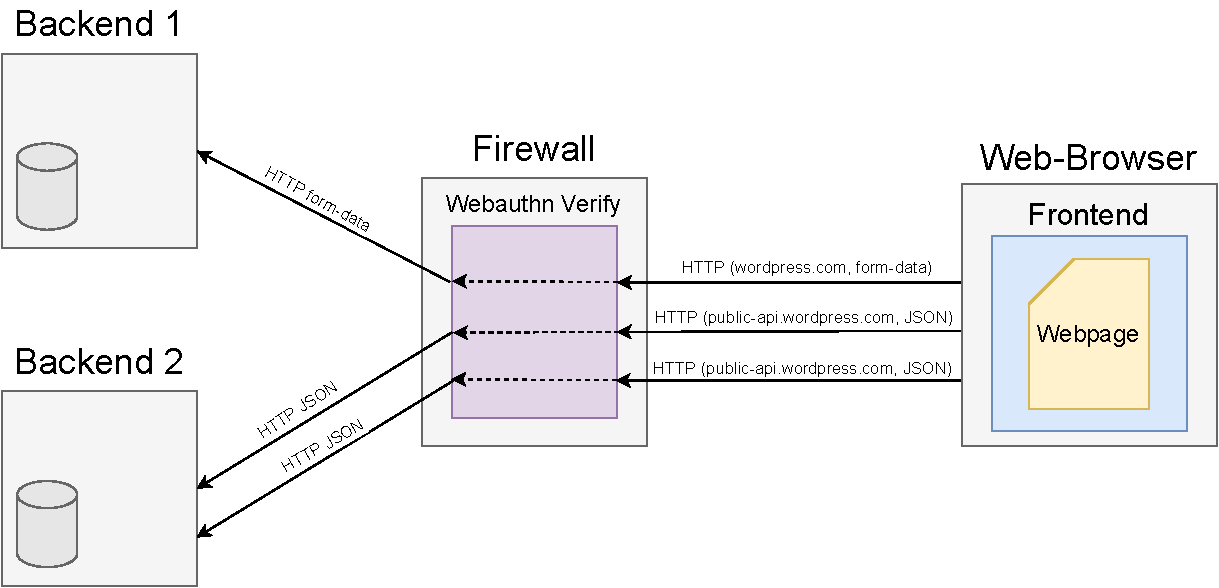
\includegraphics[width=14cm]{multitarget_calypso_drawio}
  \caption{The webauthn firewall must support two backend targets for Calypso.}
  \label{Fig:MultiTargetCalypso}
\end{figure}

Unlike the other two case studies, a point of complexity that Calypso has is that the frontend accesses multiple backends. Typically, the frontend requests to a single backend source. However, as shown in Figure~\ref{Fig:MultiTargetCalypso}, the Calypso frontend interfaces with two backend targets. WordPress has a backend for API requests, \lstinline{"public-api.wordpress.com"}, that accepts JSON payloads. Most of Calypso interacts with this backend. However, login requests go to the regular \lstinline{"wordpress.com"} backend which uses form-data payloads. This architecture design requirres the firewall to support multi-target proxying. Requests sent to the firewall contain their destined targets in their headers, and the firewall proxies accordingly. The firewall configuration for Calypso lists both of those target domains along with \lstinline{GetJSONInput} and \lstinline{GetFormInput} as their default input handlers respectively. 

\subsection{Login}\label{Sec:CalypsoLogin}

The webauthn firewall automatically protects a number of core webauthn routes, including the route for login, as described in Section~\ref{Sec:DefaultHandlers}. However, the Calypso project approaches login in an atypical fashion. Normally a service has a dedicated route for login. Calypso shares a login route with other operations, so HTTP requests are identified by an \lstinline{"action"} field in their payload, similarly as described in Section~\ref{Sec:CustomHandlers}. As a result, the default login handler cannot support Calypso directly. Extending the default login handler to be customizable for this one specific case would make the firewall's configuration too complicated. Rather, a custom login handler implements the Calypso login event. The login handler roughly resembles the following Go pseudo-code:

\begin{lstlisting}[float=h]
func finishLogin(w http.ResponseWriter, req *wf.ExtendedRequest) {
  action := req.Get("action")
  switch action {
    case "login-endpoint":
      // Webauthn verify the login request
      VerifyLogin(w, req)
    default:
      // Other requests go right through
      ProxyRequest(w, req)
  }
}
\end{lstlisting}

The handler listens on the \lstinline{"wordpress.com/wp-login.php"} route. It extracts the \lstinline{"action"} field in the request payload and validates the login attempt only if the action is \lstinline{"login-endpoint"}. The \lstinline{VerifyLogin} function performs the webauthn authentication and only upon successful verification does it allow the request to proceed through the firewall. Otherwise, all other requests are proxied through with no additional checks.

\subsection{Secured Routes}\label{Sec:CalypsoSecuredRoutes}

Table~\ref{Table:CalypsoSecuredRoutes} lists the secured operations of Calypso with a sample authentication message for each. The domain specific language supports Calypso well; every operation listed is secured using the domain specific language. This array of protected operations demonstrates the flexibility of the domain specific language.

\begin{table}[h]
\centering

\begin{tabular}{ m{5cm} m{9cm}  } 
 \hline
 Operation & Authentication Message \\ 
 \hline \hline

 Update Profile Settings & \lstinline{"Save the profile settings: Espanol Public"} \\ \hline

 Invite New Users to Site & \lstinline{"Invite new user(s): damian, durian, dominic"} \\ \hline

 Change Site Address & 
%% TODO: Figure out how to remove numbering and frame
 \begin{lstlisting} 
"Change site address
   from: calypso.localhost
   to: mytravels.blog.com"
\end{lstlisting} 
\\ \hline

 Change Site Theme & \lstinline{"Change theme to: Tangerine Orange"} \\ \hline

\end{tabular}
\caption{The operations of Calypso secured by transaction authentication.}
\label{Table:CalypsoSecuredRoutes}
\end{table}

Certain domain specific programs have multiple context retrievals. Others have multiple format tags to fill, and one program requires a special formatting function. Apart from the custom login handler, there is no case where a custom handler is necessary. 
The ``Invite New Users to Site'' route receives HTTP request containing an array of elements that need to be comma separated in the authentication message. Rather than implementing a custom handler for this minor inconvenience, the \lstinline{Apply} domain specific operation described in Table~\ref{Table:DSL_GetterOperations} resolves this problem. It enables Go code to be used within a domain specific program to a limited extent. The following is a domain specific program for inviting new users to administer a WordPress blog.

\iffalse
all of the routes in Calypso are protected using the DSL. 
\fi

\begin{lstlisting}[float=h]
firewall.Secure("POST", "/rest/{version}/sites/{site_id}/invites/new", 
  firewall.Authn("Invite new user(s): %v",
  wf.Apply(func(args ...interface{}) (interface{}, error) {
    invitees := args[0].([]string)
    return strings.Join(invitees, ","), nil
  }, wf.GetArray("invitees")),
))
\end{lstlisting}

The \lstinline{Authn} operation string formats the argument of \lstinline{wf.GetArray("invitees"))} with a Go closure passed to \lstinline{Apply}.

\section{Gogs}

Gogs is a server-side rendered self-hosted Git web service \cite{TODO-gogs}. A server-side rendered web-application presents its own set of challenges to the webauthn firewall. Section~\ref{Sec:ProxyingRequests} explains how the firewall has to be the end-point interacting with the user's web-browser. The firewall must obtain the context from the Gogs backend. The backend does not, however, conveniently expose context routes like RESTful backends as discussed in Section~\ref{Sec:Conduit_ContextRetrieval}.

%% 
%% \iffalse
%% Apart from that, context must be served by the Gogs backend. 
%% \fi
%% 

\subsection{Intrusive Webauthn}

The Gogs web service was the first of the three case-studies. Before the webauthn firewall became a mature idea, part of Gogs was secured in the traditional, intrusive fashion described in Section~\ref{Sec:StatusQuo}. This work is redone using the webauthn firewall approach once it proved itself as a prospective design approach.

The two main challenges with integrating webauthn into Gogs intrusively are the database adapter and organizational difficulties. Webauthn needs a database table to record entries of users' public key credentials. Simply creating a new table in Gogs requires writing a custom database adapter for that table and modifying the codebase in a number of separate locations. Furthermore, the handlers for various Gogs routes are spread throughout the code. Keeping track of which routes are webauthn secured becomes increasingly more difficult as more routes are protected.

%% 
%% \iffalse
%% The intrusive approach was abandoned once the firewall proved itself a prospective mechanism and all of the work redone.
%% \fi
%% 

\subsection{Context Retrieval}

A downside to server-side rendering web services when compared to RESTful services when it comes to webauthn firewall integration is the lack of pre-built context routes. Effectively, the API routes in the RESTful backend services act as the context routes. Gogs, being a server-side rendering backend, must be modified to include those context routes. Some Gogs routes need additional context to retrieve objects such as a \lstinline{"repository"} or \lstinline{"webhook"}. Gogs serves this context information out of a \lstinline{"server_context/<type>/<args>"} route. The \lstinline{<type>} refers to what type of object is being requested (e.g., repository, webhook, etc.). Each context type has its own handler in Gogs, which interprets the \lstinline{<args>} to retrieve the correct context object.

%% 
%% \iffalse
%% As the Gogs routes get webauthn protected, becomes more evident which 
%% \fi
%% 

\subsection{Secured Routes}

While integrating webauthn into Gogs during the case study, every HTTP route of the web service is categorized whether it should be protected by transaction authentication or not. This judgment is made by weighing the cost versus the benefit of protecting that route. Protecting a route is not free, most heavily affecting the user experience. Routes are protected if the harm due to malicious hijacking justifies the burden to the user's experience.

Table~\ref{Table:GogsSecuredRoutes} lists the secured operations with a sample authentication message for each. It presents an overview for the types of operations that could warrant webauthn transaction authentication.

\begin{table}[h]
\centering

\begin{tabular}{ m{5cm} m{9cm}  } 
 \hline
 Operation & Authentication Message \\ 
 \hline \hline

 Delete Repository & \lstinline{"Confirm repository delete: damian/JS-OS"} \\ \hline

 Add SSH Key & \lstinline{"Add SSH key named: Damian's Laptop"} \\ \hline

 Delete SSH Key & \lstinline{"Delete SSH key named: Damian's Laptop"} \\ \hline

 Update Profile Settings & 
%% TODO: Figure out how to remove numbering and frame
 \begin{lstlisting} 
"Confirm profile details:
   username damian
   email damianb@mit.edu"
\end{lstlisting} 
\\ \hline

 Set Primary Email & \lstinline{"Confirm new primary email: damianb@alum.mit.edu"} \\ \hline

 Change Password & \lstinline{"Confirm password change"} \\ \hline

 Leave Repository & \lstinline{"Leave repository named: JS-OS"} \\ \hline

 Delete App Access Token & \lstinline{"Delete App named: Gogs-Watcher-App"} \\ \hline

 Publish New Release &
%% TODO: Figure out how to remove numbering and frame
 \begin{lstlisting} 
"Publish release named: Version 4.20
   File names: release.tar.gz, release_x86"
\end{lstlisting} 
\\ \hline

  Delete Web-Hook & \lstinline{"Delete webhook for: URL gogswatcher.app.com"} \\ \hline

\end{tabular}
\caption{The operations of Gogs secured by transaction authentication.}
\label{Table:GogsSecuredRoutes}
\end{table}

\subsection{Custom Handlers}\label{Sec:Gogs_CustomHandlers}

As with the other case-studies, most of the routes are simple and easy to secure using the domain specific language. At most they require a context retrieval to fill a single format tag. Within the Gogs service, the ``Delete Repository'' and ``Set Primary Email'' operations in Table~\ref{Table:GogsSecuredRoutes} each share the same HTTP route for multiple different HTTP operations. Similarly to the login route of Calypso discussed in Section~\ref{Sec:CalypsoLogin}, requests have an \lstinline{"action"} field in their payload that delineates the operation type. Only certain actions warrant being transaction authenticated. Custom handlers are used in these cases, to parse the \lstinline{"action"} field and webauthn secure only when necessary.

 %% 
%% \iffalse
%% there are a number of routes such as the ``Delete Repository'' that are shared by multiple HTTP operations.

%% publishing a new release. 
%% \fi
%% 

Gogs requires a more involved custom handler for protecting the ``Publish New Release'' operation. The files associated with a new release are contained as UUIDs in the HTTP request. So each file needs context retrieval to retrieve the file name, which then must be comma separated in the format string. Rather than expressing this series of operations and formatting in an \lstinline{Apply} operation like with Calypso in Section~\ref{Sec:CalypsoSecuredRoutes}, it is easier to drop down to a custom handler function. The following code snippet is Go pseudo-code for the custom handler.

\begin{lstlisting}[float=h]
func publishNewRelease(w http.ResponseWriter, r *wf.ExtendedRequest) {
  title := r.Get("title")
  uuids := r.Request.Form["files"]

  names := []string{}
  for _, uuid := range uuids {
    append(names, r.GetContext("attachment", uuid)["Name"].(string))
  }

  authText := fmt.Sprintf("Publish release named: %v", title)
  authText += fmt.Sprintf("\nFile names: %s", strings.Join(names, ", "))

  handlerFn := firewall.Authn(authText)
  handlerFn(w, r)
}
\end{lstlisting}

This handler constructs an authentication message from the \lstinline{"title"} of the release and all of the included attachment file names. For the attachment file names, the handler must translate the UUIDs into contextualized attachment objects and then look up the \lstinline{"Name"} fields.

%% 
%% \iffalse
%% Essentially, the firewall assumes the roles of the frontend in the RESTful use-cases. 

%% of the \lstinline{"Name"} fields for every attachment UUID of the new relase
%% \fi
%% 

%% This is an example first chapter.  You should put chapter/appendix that you
%% write into a separate file, and add a line \include{yourfilename} to
%% main.tex, where `yourfilename.tex' is the name of the chapter/appendix file.
%% You can process specific files by typing their names in at the 
%% \files=
%% prompt when you run the file main.tex through LaTeX.

\chapter{Evaluation}\label{Chap:Evaluation}

%% 
%% \iffalse
%% They put in concrete terms all of the advantages of the WebAuthn firewall discussed throughout this thesis. 
%% \fi
%% 

This chapter presents evaluation metrics for the three case studies of \sys{}. The principal evaluation criteria focus on simplicity, organization, ease-of-use and performance overhead of \sys{} by answering the following questions:

\begin{itemize}[nosep]
\item What is the complexity of using \sys{}? (Section~\ref{Sec:FirewallConfigOverallComplexity})

  \begin{itemize}[nosep]
    \item What is the breakdown of the configuration file? (Table~\ref{Table:EvaluationOverallComplexity})
    \item How much incremental work does it take to secure a new route? (Figure~\ref{Fig:IncrementalComplexity})
  \end{itemize}

\item How much does a web service's frontend code need to be modified? (Section~\ref{Sec:FrontendModifications})

\item How do the changes to a web service's backend compare when integrating WebAuthn with \sys{} versus intrusively? (Section~\ref{Sec:BackendModifications})

\item What is the performance overhead of \sys{}? (Section~\ref{Sec:PerformanceOverhead})

\end{itemize}



\section{WebAuthn Firewall Configuration Metrics}

Each of the three case studies has its associated WebAuthn firewall configuration file. The number of lines of code of this file is a proxy measurement to evaluate the complexity and ease-of-use of \sys{}. 

\subsection{Overall Complexity}\label{Sec:FirewallConfigOverallComplexity}

%% 
%% \iffalse
%% lists the contents of a configuration file
%% \fi
%% 

The total configuration file size evaluates the overall complexity of configuring \sys{} and is shown in Table~\ref{Table:EvaluationOverallComplexity}, sub-divided into four categories:

\begin{itemize}[nosep]

\item Configuration parameters as discussed in Section~\ref{Sec:ConfigurationParameters}

\item Context retrieval functions as discussed in Section~\ref{Sec:ContextRetrieval}

\item Domain specific language and custom route handlers as discussed in Sections~\ref{Sec:DomainSpecificLanguage} and~\ref{Sec:CustomHandlers}

\item Miscellaneous code such as extraneous syntax and boilerplate code

\end{itemize}

%% 
%% \iffalse
%% The file sizes and the respective four-way breakdown illustrate the overall and itemized complexity of using \sys{}.
%% \fi
%% 

\begin{table}[h]
\centering

\begin{tabular}{ m{4.5cm} m{6cm}  } 
 \hline
 Case Study & Configuration File Lines of Code \\ 
 \hline \hline

 Conduit & 245 \\ \hline

 \quad Config Parameters & \quad 17 \\ \hline

 \quad Context Retrieval & \quad 117 \\ \hline

 \quad Route Handlers & \quad 49 \\ \hline

 \quad Miscellaneous & \quad 62 \\ \hline \hline

 Calypso & 253 \\ \hline

 \quad Config Parameters & \quad 22 \\ \hline

 \quad Context Retrieval & \quad 92 \\ \hline

 \quad Route Handlers & \quad 81 \\ \hline

 \quad Miscellaneous & \quad 58 \\ \hline \hline

 Gogs & 257 \\ \hline

 \quad Config Parameters & \quad 22 \\ \hline

 \quad Context Retrieval & \quad 51 \\ \hline

 \quad Route Handlers & \quad 126 \\ \hline

 \quad Miscellaneous & \quad 58 \\ \hline

\end{tabular}
\caption{A breakdown of the configuration file size for each case study. Each total is broken down into four categories with their respective lines of code contributions.}
\label{Table:EvaluationOverallComplexity}

\end{table}

The firewall configuration file is the sole source of customization that dictates how the firewall interacts with a specific web service. Both Calypso and Gogs are production web services. Considering that they are secured by \sys{} within approximately 250 lines of code, this supports the claimed advantages of the firewall's simplicity and organization. 

\subsection{Incremental Complexity to Secure a Route}

%% 
%% \iffalse
%% Conduit being the smallest and simplest web service has the smallest route handler cost. Gogs, on the opposite end of the spectrum, naturally has the largest cost. Since most routes may be secured using the domain specific language, the increase in route handler complexity increases slowly.
%% \fi
%% 

The configuration parameters, context retrieval and miscellaneous code are more or less fixed costs to the configuration file's complexity. Only the route handlers scales with the size of the service being secured. Figure~\ref{Fig:IncrementalComplexity} plots the frequencies of lines of code needed to secure a new route among all three case studies. The bar chart can be partitioned into two clear clusters at approximately the 20 lines of code per route handler boundary. The bars on the left side with fewer than 20 lines correspond to uses of the domain specific language. The handlers greater than 20 lines of code are solely the custom handlers. It is natural to expect this divide since the custom handlers by nature perform more involved processing of a request than the DSL handlers and thus use more lines of code.

%% 
%% \iffalse
%%  where the lower end of lines of code per route handler, the bars on the left who represent routes with less than approximately 20 lines of code, correspond to uses of the domain specific language. 
%% \fi
%% 

\begin{figure}[h]
  \centering
  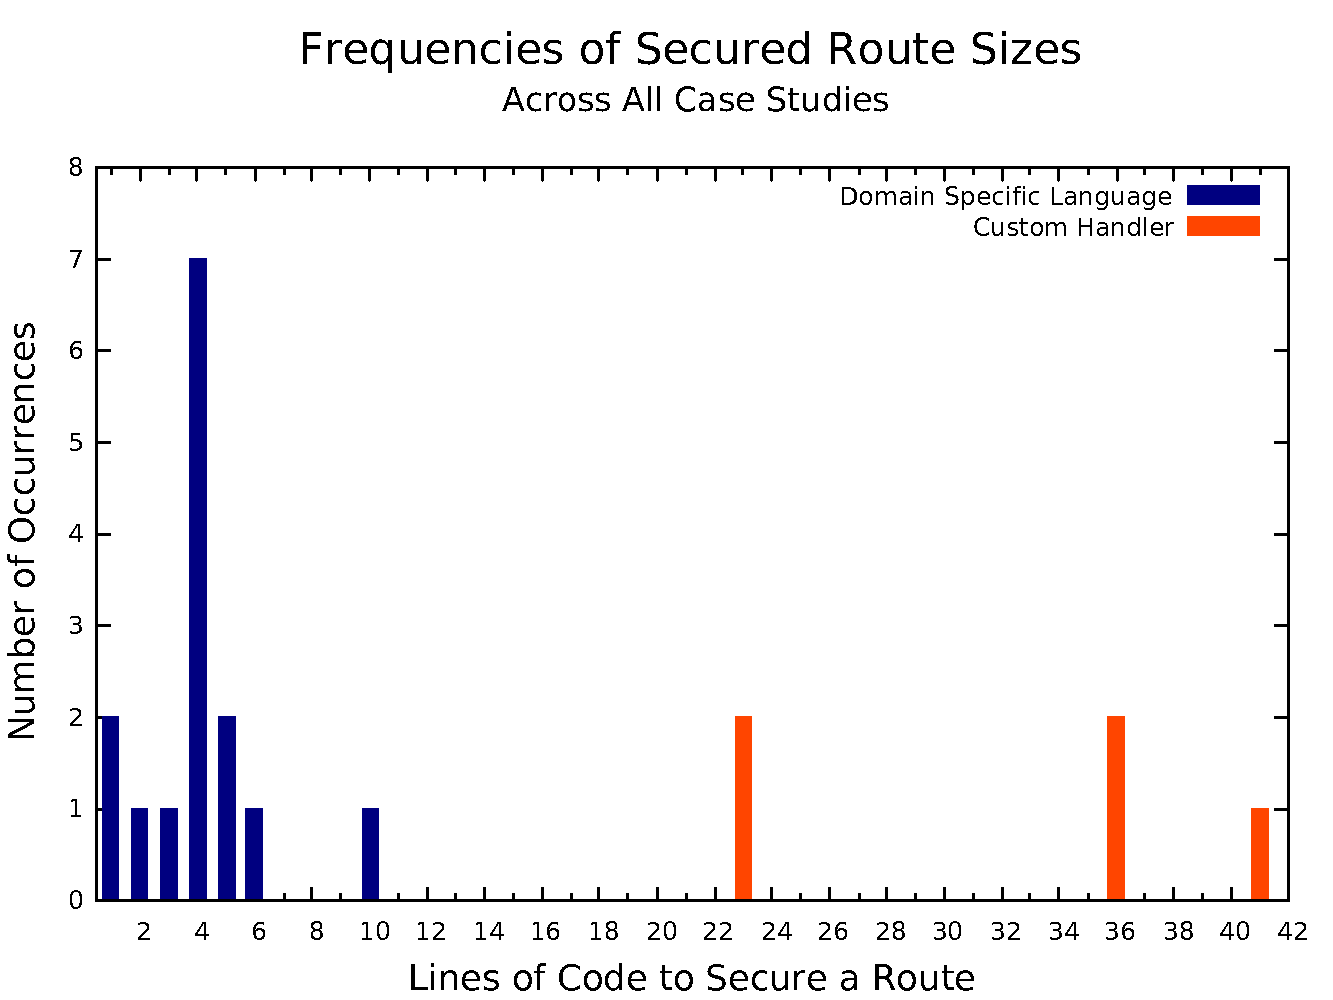
\includegraphics[width=13.5cm]{./plots/linesofcode}
  \caption{The frequencies of lines of code to secure a route with transaction authentication. The majority of the routes can be secured in 10 lines or less.}
  \label{Fig:IncrementalComplexity}
\end{figure}

This chart also evidently demonstrates that most of the routes may be secured using only the domain specific language. Of all 20 routes secured among all three case studies, only 5 required a custom handler. This means that 75\% of the routes could be captured by the domain specific language. The average domain specific program to secure a route is 4 lines of code, and the average custom handler is 32 lines of code. The total weighted average to secure a route is 11 lines of code.

%% 
%% \iffalse
%%  the domain specific language excises all of the boilerplate code wheras not handled directly in the custom handlers

%% , and they are secured using

%% The size of this configuration file and how much

%% A source of complexity when using the webauthn firewall is its configuraiton. These evaluation metrics demonstate that the firewall is 

%% In order to use the webauthn firewall on a web service, it must be configured. 

%% The total size, number of changes and 

%% Simplicity and organization

%%  are the main evaluation criteria.
%% the benefits of using the firewall to integrate webauthn into a web service. 
%% \fi
%% 

\section{Frontend Modifications}\label{Sec:FrontendModifications}

The frontend of a web service must be modified slightly when integrating WebAuthn, regardless of whether the WebAuthn firewall is in use or not. The frontend issuing the WebAuthn operation must adhere to the protocol specification life cycle as described in Chapter~\ref{Chap:WebauthnTransactionAuthentication}. Table~\ref{Table:EvaluationsFrontendModifications} lists the total number of code changes for each frontend of the case studies. For every case, the number of changes all exceed the sizes of the WebAuthn firewall configuration files.

\begin{table}[h]
\centering

\begin{tabular}{ m{4.5cm} m{6cm}  } 
 \hline
 Case Study & Frontend Lines of Code Changes \\ 
 \hline \hline

 Conduit & 289 \\ \hline

 Calypso & 402 \\ \hline

 Gogs & 570 \\ \hline

\end{tabular}
\caption{The number of code changes performed on each frontend of the case studies in order to support WebAuthn transaction authentication.}
\label{Table:EvaluationsFrontendModifications}
\end{table}

%% 
%% \iffalse
%% , but rather simple and monotonous
%% \fi
%% 

%% TODO: Not only gogs, but the overall average?
These code changes are not complex. There is boilerplate code delegated to a JavaScript library. Its contents are not included in the lines of code measurements, but its import and usage within the frontend is. The nature of protecting an operation with WebAuthn on the frontend involves making a few library calls, error handling and piecing together the authentication message from the HTML data present. For example, each Gogs operation secured by WebAuthn involves on average 54 lines of code changes to the frontend. 

%% 
%% \iffalse
%% This includes the code to correctly format and encode data fields.

%% The boilerplate code is offloaded to a JavaScript library, but the library calls as well as piecing together the authentication message make up those changes.

%% \fi
%% 

\section{Backend Modifications}\label{Sec:BackendModifications}

A significant advantage to using \sys{} over integrating WebAuthn intrusively into a web service is the lack of modifications needed to the backend. Table~\ref{Table:EvaluationsBackendModifications} demonstrates this fact --- using \sys{} is not invasive to the backend.

\begin{table}[h]
\centering

\begin{tabular}{ m{4.5cm} m{6cm}  } 
 \hline
 Case Study & Backend Lines of Code Changes \\ 
 \hline \hline

 Conduit & 0 \\ \hline

 Calypso & 0 \\ \hline

 Gogs & 169 \\ \hline

\end{tabular}
\caption{The number of code changes performed on each backend of the case studies in order to support the WebAuthn firewall.}
\label{Table:EvaluationsBackendModifications}
\end{table}

The RESTful case studies, Conduit and Calypso, require no backend modifications. The Gogs case study, which is server-side rendered, only needs modifications to supply context. 

Before \sys{} became a mature idea, Gogs was partly WebAuthn secured intrusively. The intrusive Gogs case study protects 5 routes whereas the WebAuthn firewall study of Gogs covers 11 routes. Nevertheless, even with fewer routes protected, the invasive nature of securing Gogs is unmistakable. Table~\ref{Table:EvaluationsComplexityDiffIntrusiveFirewall} backs this claim up plainly. The intrusive Gogs implementation is significantly more complex and more spread throughout Gogs than the WebAuthn firewall approach.

\begin{table}[h]
\centering

\begin{tabular}{ m{5cm} m{4.5cm} m{4.5cm}  } 
 \hline
 & Backend Lines Changed & Backend Files Modified \\ 
 \hline \hline

 Intrusive Gogs & 1293 & 18 \\ \hline

 WebAuthn Firewall Gogs & 169 & 5 \\ \hline


\end{tabular}
\caption{Comparing the complexity differences between intrusive and WebAuthn firewall integration.}
\label{Table:EvaluationsComplexityDiffIntrusiveFirewall}
\end{table}

Many of the additional lines of code for the intrusive WebAuthn integration of Gogs come from all of the plumbing code needed in to support and run WebAuthn. WebAuthn needs its own database table with entries to record registered users. The backend must support WebAuthn registration and login. It must also include the WebAuthn code that verifies transaction authentication events. All of these functionalities come with \sys{} for free, which explains the large reduction in backend complexity when using \sys{}.

\sys{} also reduces the amount of boilerplate code required to secure a new route. Gogs secured intrusively takes on average 87 lines of code per new route. The firewall has on average 11 lines per new route.

%% 
%% \iffalse
%% minimally invasive

%% Not all of the routes covered by the webauthn firewall case study of Gogs were done intrusively, but only the handful secured are enough to outline the minimal.
%% \fi
%% 

\section{Performance Overhead}\label{Sec:PerformanceOverhead}

\begin{figure}
  \centering
  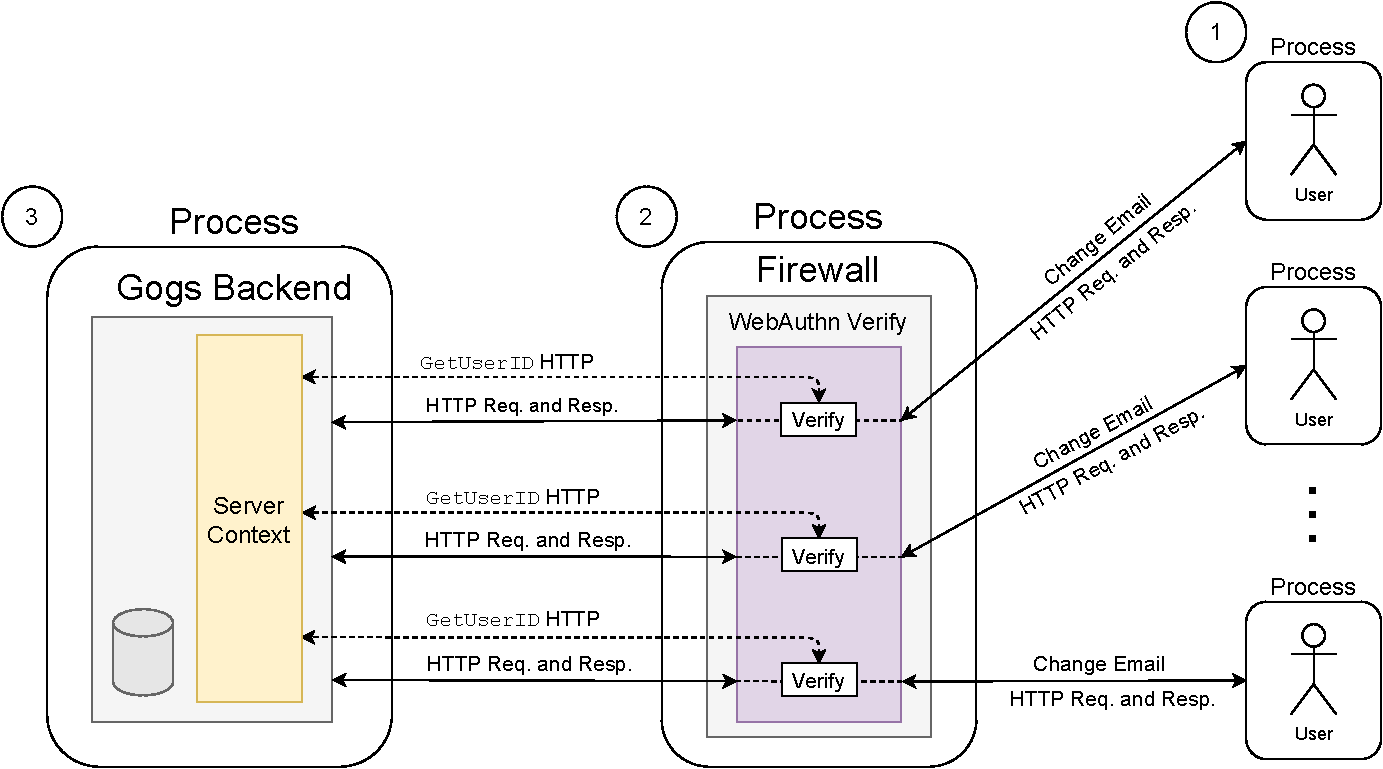
\includegraphics[width=\textwidth]{./performance_experiment_drawio}
  \caption{The experiment setup to measure the performance overhead of \sys{} under load.}
  \label{Fig:PerformanceExperimentSetup}
\end{figure}

\sys{} acts as a gatekeeper between the frontend and backend. It naturally adds some performance overhead to the whole system. This evaluation experiment measures the performance overhead for securing Gogs with \sys{} under load to see how well it scales. 

%% 
%% \iffalse
%%  timing the latency of each request to run to completion. 
%% \fi
%% 

The hardware for this experiment is a quad-core Intel i7-6600U CPU @ 2.60GHz laptop machine. Figure~\ref{Fig:PerformanceExperimentSetup} illustrates the setup used to collect the performance data. The firewall and Gogs web server run in separate operating system processes. Each trial to collect performance run times initializes a given number of users running in their own operating system processes. Each user proceeds to sequentially send 300 POST requests to the ``Change Email'' route as quickly as possible. This workload generation is performed as a closed-loop system, where each user sends a new HTTP request only when their previous request comes back with an HTTP response. The latency of each request is the elapsed time measured for the request to return a response. The data point for the trial is the $95^{th}$ percentile of the running times tail. When there are many users sending requests simultaneously, there is contention among them which accounts for the increase in latency.

%% TODO: Make sure colors match up
Three different scenarios are tested and the results reported in Figure~\ref{Fig:PerformanceOverhead}. The blue line measures the request latencies for using \sys{} on users that have WebAuthn enabled. The orange line measures the request latencies for \sys{} on users without WebAuthn enabled. The difference between these two lines is the overhead of validating a WebAuthn transaction versus simply letting the request pass through. The red line measures the latencies of sending these requests directly to the Gogs server.

\begin{figure}[h]
  \centering
  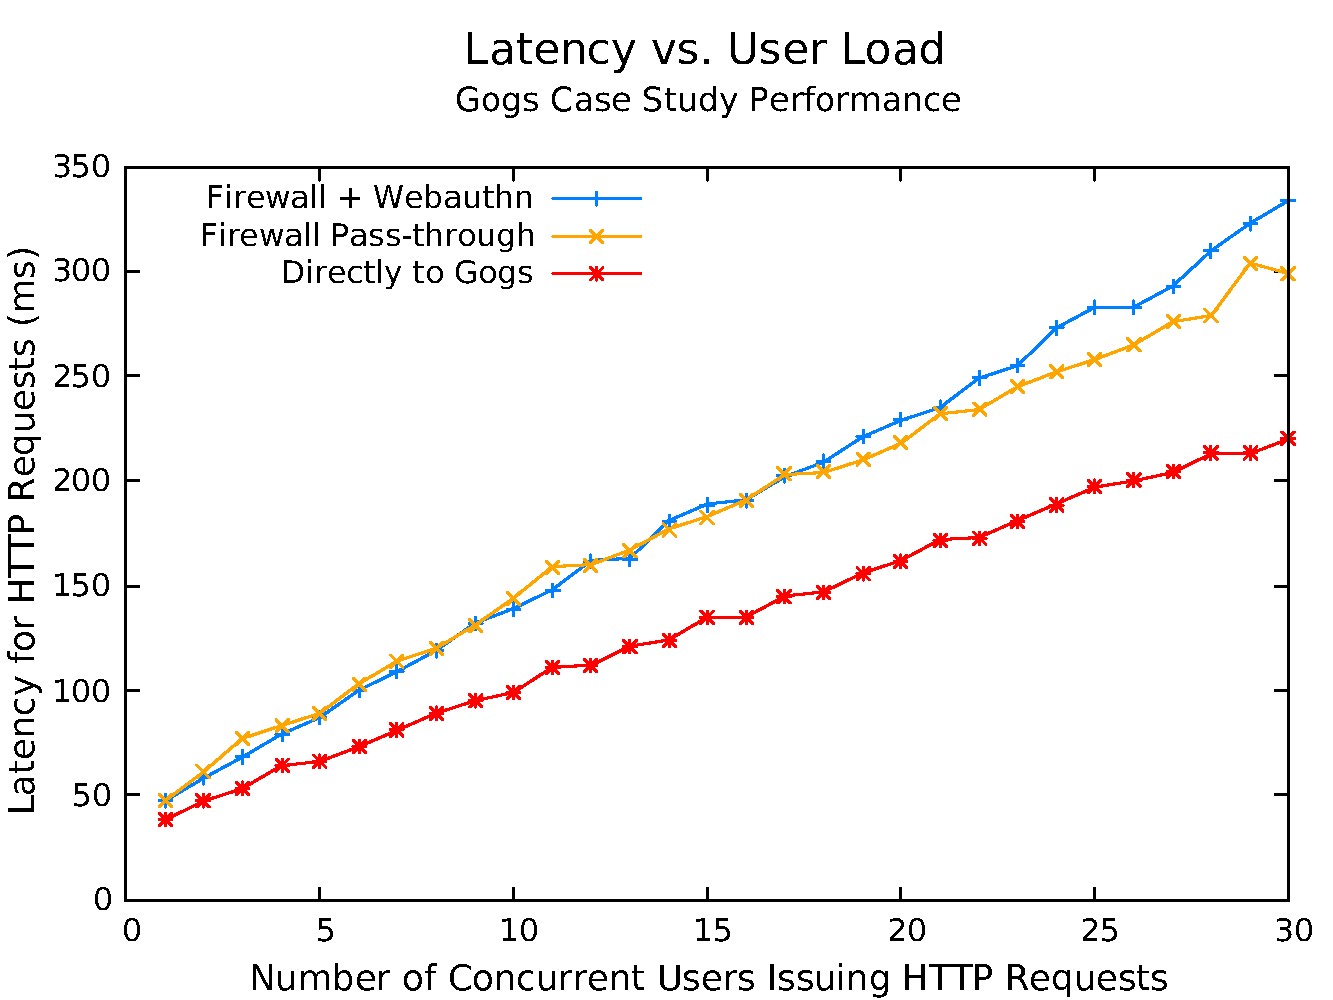
\includegraphics[width=13.5cm]{./plots/runtimes}
  \caption{The 95\textsuperscript{th} percentile run times of three different Gogs setups under load. The x-axis is the number of users issuing requests concurrently, and the y-axis is the run time latency in milliseconds. The three experiments are: using \sys{} with WebAuthn enabled, using \sys{} with WebAuthn disabled, issuing requests directly to the Gogs server without WebAuthn transaction authentication. There is a latency penalty to using the WebAuthn firewall.}
  \label{Fig:PerformanceOverhead}
\end{figure}

As seen in Figure~\ref{Fig:PerformanceOverhead}, the blue and orange line remain tightly together meaning that there is little overhead from the actual validation of a WebAuthn transaction. Rather there is a significant gap between the lower red line representing the direct connection and the upper blue and orange lines representing the firewall setups. This discrepancy arises from the implementation of the \lstinline{GetUserID} function within the Gogs firewall. The \lstinline{GetUserID} is a configurable function described in Section~\ref{Sec:ConfigurationParameters} which identifies the current user of a request received by \sys{}. 

\sys{} uses the current user information to determine, for every incoming HTTP request, whether that user has WebAuthn enabled in order to verify the transaction accordingly if so. In Gogs, the user of a request is identified by a session ID, which only the backend can translate to a user ID. Therefore, the \lstinline{GetUserID} for the Gogs firewall must send an HTTP GET request to the backend to retrieve the user ID. As depicted by the dashed request lines in Figure~\ref{Fig:PerformanceExperimentSetup}, every request that passes through the firewall invokes an additional HTTP request, accounting for the substantial overhead when using the firewall. Under the 30 user load, the additional overhead of this \lstinline{GetUserID} HTTP request adds approximately 70 milliseconds to the overall latency. This is visible in the non-negligible gap between the lower red line and the upper blue and orange lines.

The \lstinline{GetUserID} function is specific to the web service, and it is possible to design the software to avoid the additional HTTP call. The Conduit web service, for example, uses JSON Web Tokens (JWT) in order to identify the current user of an HTTP request. In this setup, the user ID is simply included in a signed JSON object with the request. \sys{} can simply parse this data object and extract the identifier directly without any additional HTTP requests. Under such a setup, the latency discrepancy between using \sys{} and the direct scenarios should diminish significantly.

%% 
%% \iffalse
%% There are three measurements

%% There naturally is a performance overhead suffered because of the .

%%   it naturally does add performance overhead.

%% Despite all of the advantages laid out by the webauthn firewall,
%% \fi
%% 

%% This is an example first chapter.  You should put chapter/appendix that you
%% write into a separate file, and add a line \include{yourfilename} to
%% main.tex, where `yourfilename.tex' is the name of the chapter/appendix file.
%% You can process specific files by typing their names in at the 
%% \files=
%% prompt when you run the file main.tex through LaTeX.

\chapter{Discussion and Future Work}\label{Chap:DiscussionAndFutureWork}

This chapter makes a number of observations on transaction authentication discovered over the course of this research. 

\section{Applications of Transaction Authentication}

Transaction authentication is not without its limitations. There are use cases that make perfect sense for this authentication extension, which fit nicely within its specification and capabilities. Other cases may not lend themselves well to transaction authentication. The complexity of the authentication message displayed is a key determining factor for what makes a good versus poor use case.

%% 
%% \iffalse
%% There are other use cases that are possible to be secured, but begin to suffer with ease of use. 

%% However not all possible use cases are as clean to
%% \fi
%% 

\subsection{Good Use Cases}

Good use cases of transaction authentication are those where the authentication message is short, simple and easy to comprehend by a user. The contents being displayed should also be human-readable in nature. Names and titles are easily recognizable by a human. A cryptographic key, albeit displayable, is much less human-friendly. 

An example from Gogs is the delete repository action. It is secured with the authentication message: \lstinline|"Confirm repository delete: {username}/{reponame}|. From this message, it should be immediately evident to a user what the operation to be performed is. 

A short authentication message is less likely to be misinterpreted by the user. Additionally, a hardware authenticator device is likely to have a relatively small display. So shorter authentication messages are better fit for this restrictive display medium. 

%% 
%% \iffalse
%% To benefit the most from transaction authentication, a dedicated hardware device should perform the cryptographic attestation discussed in Section~\ref{Sec:CryptographicAttestation}. 
%% \fi
%% 

\subsection{Poor Use Cases}

A poor use case is one where it is possible to use transaction authentication, but it is rather clunky and disruptive to the user experience. Three general classes of such problems are as follows:

\begin{itemize}[nosep]

\item There is a lot of context to authenticate. One example is a big form that needs transaction authentication. This form is unlikely to all fit on the hardware authenticator's display. Also, even when only one aspect of the form is modified, all of the entries must be displayed to the user since they all are sent over in the HTTP request.

\item The contents being displayed are not friendly for human readability. Examples include SSH keys, cryptographic hashes, and Git hooks code blocks. These can be displayed, but are burdensome for the user to verify.

\item The context media is difficult or impossible to meaningfully be displayed. Rich media such as images or audio clips fully depend on the hardware authenticator's physical capabilities. Binary uploads have no good way of being displayed to the user at all. For example, the Gogs route to publish a new release as discussed in Section~\ref{Sec:Gogs_CustomHandlers} has no way to validate the binary contents being uploaded.

%% 
%% \iffalse
%% An example route in this category would be the Gogs new release upload form.
%% \fi
%% 

\end{itemize}

%% 
%% \iffalse
%% make for poor use cases of transaction authentication. 
%% \fi
%% 

\subsection{Inapplicable Use Cases}

Transaction authentication defends against unauthorized and unwanted operations on a user's account. However, under the threat model defined in Section~\ref{Sec:ThreatModel}, it is incapable of performing any form of secure input. That means that transaction authentication cannot prevent a malicious keyboard sniffer from recording a credit card number being input during checkout or a new password being set in the account settings. Transaction authentication may prevent these events from being maliciously initiated by an adversary, but it has no means of preventing any snooping on sensitive data as it is entered into a website.

\section{RPC Isolation}

Transaction authentication is often understood as a mechanism to protect the user by defending against unauthorized operations. Intrusive integration of transaction authentication into a web service has a collateral benefit of being able to shrink the trusted computing base on the server-side. The original threat model assumes that all server code is secure. However, if a web service RPC isolates its various components internally, then only the component actually executing the given operation must be trusted. 

For example, the Gogs web sever has code and database tables pertaining to repository actions. They are independent of any other server operations and can be RPC isolated into a separate operating system process. This process is the only one with the privileges to execute repository actions, from renaming to deleting a repository. Consequently, the web server must interface with this process in order to operate on any repository. If this RPC isolated process also contains WebAuthn verification code, it can perform the transaction authentication validation on its own. Even if any other aspect of the web server were compromised, the WebAuthn protected repository requests sent to this process cannot be tampered with since they would fail the verification.

%% 
%% \iffalse
%% If transaction authentication is integrated into a web service intrusively, not 

%% However, it has the collateral benefit of being able to shrink the trusted computing base 

%% This is the case when said component is the one performing the WebAuthn verification.
%%  transaction authentication secured repository requests cannot be modified since the trusted component would fail its verification.
%% \fi
%% 

\section{Tracing Transaction Authentication \newline Subversion Opportunities}

%% 
%% \iffalse
%% is unexpectedly nuanced with the possibility to
%% \fi
%% 

Securing a route with transaction authentication requires careful planning to avoid any vulnerabilities of directly or indirectly subverting the protection. Direct subversion actively evades the transaction authentication protection. Indirect subversion tricks the user into transaction authenticating some operation that actually is undesired.

\subsection{Direct Subversion}
If the disable WebAuthn event were not transaction authentication secured, a trivial example of direct subversion is possible. The adversary could disable WebAuthn before performing any sensitive operation. To avoid this, the disable WebAuthn operation is one of the default operations protected by the firewall as discussed in Section~\ref{Sec:ConfigurationParameters}.

%% 
%% \iffalse
%% , so this hypothetical scenario cannot happen.
%% \fi
%% 

Less obvious direct subversion attacks are also possible. In Gogs, an adversary could create a new dummy user without WebAuthn enabled. Then they could add the dummy user as an owner of a target repository and perform the delete operation from the unsecured user. If not carefully protected, such as requiring transaction authentication also for adding new repository owners, this sequence of operations could subvert the protected route of repository deletion.

Direct subversion opportunities might be detectable by performing route search and analysis similar to symbolic execution. Such a system could scan the web service's code and trace all possible chains of operations that could get around the transaction authentication protection of a specific route.

\subsection{Indirect Subversion}
Indirect subversion opportunities are harder to detect since they involve a human element. These attacks trick the user into transaction authenticating a seemingly innocuous operation when actually they are authorizing something sensitive. 

An example within Gogs is the following scenario. A user has two repositories $A$ and $B$. The repository $A$ is important whereas $B$ is garbage. In this scenario, repositories may be deleted or renamed. Deletion is WebAuthn protected whereas renaming is not.

When the user decides to delete the garbage repository $B$, the adversary quickly and quietly renames $A$ to $B$ and $B$ to $A$. So by the time the user authorizes the deletion of $B$, repository $B$ is actually the important one. In doing so, the adversary hijacked the user's faithful deletion of the original garbage repository $B$ in order to delete the important repository $A$. 

%% 
\iffalse
While the user is in the process of deleting a repository $B$, 
\fi
%% 

The user believes that they are doing one operation, but in reality, they are doing a completely different and destructive other operation. Indirect subversion opportunities are difficult to notice and detect since, unlike the direct subversion opportunities, there need not be any causal links between operations. In the aforementioned example, there is no codified link between renaming a repository and its deletion. This attack purely relies on silently duping the user.

%% 
%% \iffalse
%% A trivial example of a direct subversion attack would be, if the disable WebAuthn event were not transaction authentication secured, the adversary could disable WebAuthn before performing their desired sensitive operation.
%% \fi
%% 

%% This is an example first chapter.  You should put chapter/appendix that you
%% write into a separate file, and add a line \include{yourfilename} to
%% main.tex, where `yourfilename.tex' is the name of the chapter/appendix file.
%% You can process specific files by typing their names in at the 
%% \files=
%% prompt when you run the file main.tex through LaTeX.

\chapter{Conclusion}\label{Chap:Conclusion}

This thesis presents a WebAuthn firewall architecture with the central aim of reducing the burden for integrating transaction authentication into a new or existing web service. Before this research, WebAuthn would be integrated directly into the web service's codebase, which is time consuming and difficult to maintain. The firewall approach enables an engineer to configure a ruleset for the firewall using the domain specific language and, if necessary, custom handlers. This configuration determines which HTTP requests are high-risk and which are not. The firewall processes those that are deemed high-risk and only allows them to pass through if the transaction authentication validates successfully.

Three case studies with evaluations justify the advantages of this system over integrating WebAuthn intrusively.

\begin{itemize}[nosep]
\item Complexity: The average firewall configuration file size among the case studies is approximately 250 lines of code. The average secured route for Gogs done intrusively is 87 lines of code. Considering all of the boilerplate code necessary to support WebAuthn, the firewall approach is almost 8 times more concise than the intrusive approach.

%% 
%% \iffalse
%%  It is undeniably the less complex approach to integrating transaction authentication.

%% This does not account for all of the necessary boilerplate code which the firewall handles by default. 

%%  per secured route for Gogs done intrusively, using the firewall is undeniably the less complex approach.

%% The firewall also handles all of the necessary boilerplate code resulting 
%% \fi
%% 

\item Configurability: Among the case studies, 75\% of all routes can be secured using the domain specific language in 20 lines of code or less. The average secured route requires 11 lines of code, so making adjustments to the configuration is simple and painless. 

  %% 
%% \iffalse
%% The firewall supplies the engineer with a collection of default handlers and a domain specific language to enable ease and flexibility of configuration. 
%% \fi
%% 

\item Intrusiveness: In both RESTful case studies using the WebAuthn firewall, no modifications are necessary to the backend. The Gogs case study with the firewall requires 169 lines of code changes. Contrasted to the almost 1300 lines of code change over 18 different files for the intrusive Gogs case study, the firewall is the significantly less invasive approach.

  %% 
%% \iffalse
%% to integrate WebAuthn with the firewall. Using the firewall with the server-side rendering Gogs web service requires only 169 changes, mainly for context retrieval support. Intrusively integrating WebAuthn in Gogs which requires almost 1300 code changes over 18 different files. In contrast to 169 lines of code changes, the firewall is significantly much less invasive to the web service backend.
%% \fi
%% 

\end{itemize}

The firewall does incur a performance penalty, which varies depending on the implementation details of the web service. The session ID implementation of Gogs requires that the firewall make an HTTP request in order to identify the current user issuing a request. Under heavy concurrent load, the latency penalty of the additional HTTP request is as high as 70 milliseconds.

In conclusion, the WebAuthn firewall architecture is flexible and extensible. With relatively little effort, it can equip even a production level web service with WebAuthn transaction authentication. When well tuned for performance, such a WebAuthn firewall architecture design is an appealing option for greater web security.

%% 
%% \iffalse
%% for integrating transaction authentication into a new or existing web service. Using this approach dramatically decreases the code complexity for integrating webauthn 

%% This thesis presents a webauthn firewall architecture and three case studies with evaluations to justify the benefits and advantages of this system. 

%% From the viewpoint of code complexity the firewall 

%%  presents an attractive system architecture to integrating webauthn transaction authentication into a new or existing web service. 
%% \fi
%% 

\appendix
%\chapter{Tables}

\begin{table}
\caption{Armadillos}
\label{arm:table}
\begin{center}
\begin{tabular}{||l|l||}\hline
Armadillos & are \\\hline
our	   & friends \\\hline
\end{tabular}
\end{center}
\end{table}

\clearpage
\newpage

%\chapter{Figures}

\vspace*{-3in}

\begin{figure}
\vspace{2.4in}
\caption{Armadillo slaying lawyer.}
\label{arm:fig1}
\end{figure}
\clearpage
\newpage

\begin{figure}
\vspace{2.4in}
\caption{Armadillo eradicating national debt.}
\label{arm:fig2}
\end{figure}
\clearpage
\newpage

%% This defines the bibliography file (main.bib) and the bibliography style.
%% If you want to create a bibliography file by hand, change the contents of
%% this file to a `thebibliography' environment.  For more information 
%% see section 4.3 of the LaTeX manual.
\begin{singlespace}
\bibliography{main}
\bibliographystyle{plain}
\end{singlespace}

\end{document}

